%============================================================
%  SyncAcademy – CSE 3200 System Development Project Report
%  Khulna University of Engineering & Technology
%  Strictly following the provided KUET report template
%============================================================

\documentclass[12pt,a4paper]{report}

%------------------------------------------------------------
% PACKAGES
%------------------------------------------------------------
\usepackage[T1]{fontenc}
\usepackage[utf8]{inputenc}
\usepackage{mathptmx}             % Times Roman
\usepackage{setspace}
\usepackage[top=1.2in, bottom=1.0in, left=1.2in, right=1.0in,
            headheight=15pt, headsep=0.2in, footskip=0.45in]{geometry}
\usepackage{graphicx}
\usepackage{caption}
\usepackage{titlesec}
\usepackage{tocloft}
\usepackage{fancyhdr}
\usepackage{microtype}
\usepackage{parskip}
\usepackage{array}
\usepackage{booktabs}
\usepackage{longtable}
\usepackage{tabularx}
\usepackage{hyperref}
\usepackage{url}
\usepackage{enumitem}
\usepackage{float}
\usepackage{amsmath}
\usepackage{xcolor}
\usepackage{amssymb}   % for \checkmark

%------------------------------------------------------------
% LINE SPACING  (1.5 everywhere)
%------------------------------------------------------------
\setstretch{1.5}

%------------------------------------------------------------
% PARAGRAPH SPACING
%------------------------------------------------------------
\setlength{\parindent}{0pt}
\setlength{\parskip}{6pt}

%------------------------------------------------------------
% HEADER / FOOTER
%------------------------------------------------------------
\pagestyle{fancy}
\fancyhf{}
\renewcommand{\headrulewidth}{0pt}
\fancyhead[C]{}
\fancyfoot[C]{\thepage}

\fancypagestyle{plain}{%
  \fancyhf{}
  \renewcommand{\headrulewidth}{0pt}
  \fancyfoot[C]{\thepage}
}

%------------------------------------------------------------
% CHAPTER TITLE FORMAT
% "CHAPTER I"  -> 14pt Bold Centered
% Chapter name -> 16pt Bold Centered, 1.5 line space
%------------------------------------------------------------
\titleformat{\chapter}[display]
  {\centering\fontsize{14}{21}\selectfont\bfseries}
  {CHAPTER \Roman{chapter}}
  {0pt}
  {\centering\fontsize{16}{24}\selectfont\bfseries}
\titlespacing*{\chapter}{0pt}{0pt}{24pt}

% Keep chapter heading in Roman while preserving Arabic-style figure/table numbering like 3.1, 4.2
\renewcommand{\thechapter}{\Roman{chapter}}
\renewcommand{\thefigure}{\arabic{chapter}.\arabic{figure}}
\renewcommand{\thetable}{\arabic{chapter}.\arabic{table}}
\renewcommand{\thesection}{\arabic{chapter}.\arabic{section}}
\renewcommand{\thesubsection}{\arabic{chapter}.\arabic{section}.\arabic{subsection}}

% TOC chapter entries like: CHAPTER I Introduction
\renewcommand{\cftchappresnum}{CHAPTER\ }
\renewcommand{\cftchapaftersnum}{\ }
\setlength{\cftchapnumwidth}{7em}

%------------------------------------------------------------
% SECTION  14pt Bold Left  space-before 12pt, after 6pt
%------------------------------------------------------------
\titleformat{\section}
  {\fontsize{14}{21}\selectfont\bfseries}
  {\thesection}{1em}{}
\titlespacing*{\section}{0pt}{12pt}{6pt}

%------------------------------------------------------------
% SUBSECTION  12pt Bold Left
%------------------------------------------------------------
\titleformat{\subsection}
  {\fontsize{12}{18}\selectfont\bfseries}
  {\thesubsection}{1em}{}
\titlespacing*{\subsection}{0pt}{12pt}{6pt}

\titleformat{\subsubsection}
  {\fontsize{12}{18}\selectfont\bfseries\itshape}
  {\thesubsubsection}{1em}{}
\titlespacing*{\subsubsection}{0pt}{12pt}{6pt}

%------------------------------------------------------------
% CAPTIONS  11pt Normal Centered (figure below, table above)
%------------------------------------------------------------
\DeclareCaptionFont{capfont}{\fontsize{11}{16.5}\selectfont}
\captionsetup{
  font=capfont,
  labelfont=normalfont,
  justification=centering,
  skip=12pt
}
\captionsetup[table]{position=above, skip=12pt}

%------------------------------------------------------------
% TOC
%------------------------------------------------------------
\renewcommand{\cftchapfont}{\bfseries}
\renewcommand{\cftchappagefont}{\bfseries}
\setlength{\cftbeforechapskip}{6pt}

%------------------------------------------------------------
% HYPERREF
%------------------------------------------------------------
\hypersetup{colorlinks=true,linkcolor=black,urlcolor=black,citecolor=black}

%------------------------------------------------------------
% PLACEHOLDER FIGURE HELPER
%------------------------------------------------------------
\newcommand{\placeholderfig}[2]{%
  \begin{figure}[htbp]
    \centering
    \fbox{\parbox{0.82\textwidth}{%
      \centering\vspace{1.5cm}
      \textit{[PLACEHOLDER: #1]}\\[0.4cm]
      \textit{Insert the figure / diagram here}
      \vspace{1.5cm}}}
    \caption{#2}
  \end{figure}}

%============================================================
\begin{document}
\pagenumbering{roman}

%============================================================
%  COVER PAGE  (no page number, no header)
%============================================================
\begin{titlepage}
\thispagestyle{empty}
\begin{center}

{\fontsize{14}{21}\selectfont CSE 3200: System Development Project}\\[12pt]

{\fontsize{18}{27}\selectfont\bfseries\scshape
SyncAcademy: An Academic Excellence Platform}\\

\vspace{2\baselineskip}

{\fontsize{14}{21}\selectfont By}\\

\vspace{3\baselineskip}

{\fontsize{14}{21}\selectfont\bfseries Niloy Chowdhury}\\
{\fontsize{14}{21}\selectfont Roll: 2107117}\\[10pt]
{\fontsize{14}{21}\selectfont\bfseries \&}\\[10pt]
{\fontsize{14}{21}\selectfont\bfseries Md. Tariful Islam Jony}\\
{\fontsize{14}{21}\selectfont Roll: 2107119}\\

\vspace{2\baselineskip}

%% Replace the fbox line with:
%%   
\includegraphics[width=1.14in,height=1.0in]{kuet_logo.png}

\includegraphics[width=1.14in,height=1.0in]{system_ss/kuet_logo.png}

\vspace{2\baselineskip}

\begin{spacing}{1.2}
{\fontsize{12}{14.4}\selectfont\bfseries
Department of Computer Science and Engineering\\
Khulna University of Engineering \& Technology\\
Khulna 9203, Bangladesh\\
April, 2026}
\end{spacing}

\end{center}
\end{titlepage}

%============================================================
%  TITLE PAGE  (page i)
%============================================================
\setcounter{page}{1}
\thispagestyle{plain}

\begin{center}
{\fontsize{18}{27}\selectfont\bfseries
SyncAcademy: An Academic Excellence Platform}\\
\vspace{3\baselineskip}
{\fontsize{12}{18}\selectfont By}\\
\vspace{2\baselineskip}
{\fontsize{12}{18}\selectfont\bfseries Niloy Chowdhury}\\
{\fontsize{12}{18}\selectfont Roll: 2107117}\\[6pt]
{\fontsize{12}{18}\selectfont \&}\\[6pt]
{\fontsize{12}{18}\selectfont\bfseries Md. Tariful Islam Jony}\\
{\fontsize{12}{18}\selectfont Roll: 2107119}\\
\vspace{4\baselineskip}
\end{center}

\noindent{\fontsize{12}{18}\selectfont\bfseries Supervisor:}\\[6pt]
\hspace{0.8in}{\fontsize{12}{18}\selectfont\bfseries Nabil Faiyaz Sadi, Lecturer}\\
\hspace{0.8in}{\fontsize{12}{18}\selectfont Department of Computer Science and Engineering}\\
\hspace{0.8in}{\fontsize{12}{18}\selectfont Khulna University of Engineering \& Technology}
\hfill
\begin{minipage}[t]{1.8in}
\centering
\underline{\hspace{1.8in}}\\[2pt]
{\fontsize{12}{18}\selectfont Signature}
\end{minipage}

\vfill


\begin{center}
\begin{spacing}{1.2}
{\fontsize{12}{14}\selectfont
Department of Computer Science and Engineering\\
Khulna University of Engineering \& Technology\\
Khulna 9203, Bangladesh\\
April, 2026}
\end{spacing}
\end{center}
\newpage

%============================================================
%  ACKNOWLEDGMENT  (page ii)
%============================================================
\chapter*{Acknowledgment}
\addcontentsline{toc}{chapter}{Acknowledgment}
\thispagestyle{plain}
\vspace{2\baselineskip}

All praise to Almighty Allah, whose grace and mercy enabled us to complete this project successfully. We would like to convey our deepest gratitude to our supervisor Nabil Faiyaz Sadi, Lecturer, Department of Computer Science and Engineering, Khulna University
of Engineering \& Technology, for providing invaluable guidance, constructive criticism, and unwavering support throughout every phase of development. Without the supervisor's timely direction, the scope and quality of this project would not have been achievable.

We also extend our sincere thanks to the faculty members of this Department of Computer whose teaching provided the theoretical and practical foundations upon which SyncAcademy is built. We are also very thankful to the open-source communities whose help me easy our journey.
Finally, we acknowledge the patience and understanding of our families and friends. They supported us throughout the long hours of development, debugging, and writing that this project demanded.

\vspace{2\baselineskip}
\hfill{\fontsize{12}{18}\selectfont\bfseries Niloy Chowdhury and Md. Tariful Islam Jony}
\newpage

%============================================================
%  ABSTRACT  (page iii)
%============================================================
\chapter*{Abstract}
\addcontentsline{toc}{chapter}{Abstract}
\thispagestyle{plain}
\vspace{2\baselineskip}
SyncAcademy is a smart class and materials management system that is developed as a full-stack, AI-driven system. In this project we  particularly focused on the academic processes of Khulna University of Engineering \& Technology (KUET). Our current academic management systems often suffer from fragmentation where study materials, examinations, communication and administrative tasks are handled through separate platforms. This lack of integration leads to inefficiencies, poor coordination and reduced engagement. By addressing these challenges, our project  has been developed as a unified academic management and learning system. It integrate multiple educational functionalities into a single platform. Its architecture is based on a three-tier web app. Firstly, React 18 and Material UI 5 frontend with student, teacher, and administrator role-based dashboards. Secondly,  a Node.js 18 and Express 4 REST API server based on Mongoose 9, which is linked to MongoDB. Lastly, an AI services which is a locally hosted Ollama large language model with a Hugging Face sentence integration pipeline. The roles of users are determined automatically at KUET institutional email domains during registration: students are sent stud.kuet.ac.bd addresses administrators and teachers receive @kuet.ac.bd addresses. The summary of main features of this project are: Semantic searching for materials, Retrieval Augmented Generation (RAG) based AI support, role based course management, a course announcement stream with auto-generated enrollment codes,nested comments, replies, attachments, and pin support; an assignment and submission system: due-date late detection, teacher feedback, uploaded evaluated script PDF, result sheet support; an AI quiz generator that generates multiple-choice questions based on chunks of uploaded course materials; a manual quiz-creator with timing and accessibility etc. The system is implemented in the site:\url{https://syncacademy.onrender.com}. We tried to follow standard software development practices for scaling  in future improvements. Overall, SyncAcademy is a simple and effective solution for our academic challenges and it creates a more organized and user friendly learning experience for all users.

\newpage

%============================================================
%  TABLE OF CONTENTS
%============================================================
\tableofcontents\newpage

%============================================================
%  LIST OF TABLES
%============================================================
\listoftables\newpage

%============================================================
%  LIST OF FIGURES
%============================================================
\listoffigures\newpage

%============================================================
%  MAIN MATTER
%============================================================
\pagenumbering{arabic}
\setcounter{page}{1}

%============================================================
\chapter{Introduction}
%============================================================

\section{Introduction}

Contemporary universities are increasingly turning to online platforms to administer courses, student engagement, and formative assessment. Nevertheless, the tools most commonly used in this space such as Google Classroom, Drive and others are share a common limitation: they primarily serve as passive delivery channels. Assignments are collected and files are uploaded, but the platforms do not offer any intelligence to assist students in locating appropriate materials, understanding complex concepts in context or identifying their knowledge gaps.

SyncAcademy is a web-based smart classroom management system designed to address this limitation. It provides the full feature set of platforms like Google Classroom while integrating three AI-powered subsystems: semantic material search, a Retrieval-Augmented Generation (RAG) AI Tutor, and an adaptive recommendation engine based on Knowledge Tracing—all unified within a single platform tailored specifically to KUET’s academic processes. The project was developed as part of the System Development Project course (CSE 3200) by two KUET CSE students.



\section{Background and Problem Statement}
The KUET learning environment has several causes to make our project relevent. here email addresses: each student, teacher, and administrator has a distinct domain suffix. It enables automatic role assignment without manual intervention. Evaluation in engineering programs involves a wide range of formats, including written assignments, oral vivas, group presentations, and thesis defenses. Additionally, teaching assistant support is limited relative to class sizes which can making AI-assisted tutoring and structured self-study guidance particularly important.

SyncAcademy is motivated by four key problems. Firstly, material discovery that means when a course provides a collection of lecture slides, notes, and references, students searching for content on a specific concept must rely on manual search rather than intelligent retrieval. Second, personalized guidance refers to existing classroom tools do not adapt content recommendations based on what a student has or has not yet mastered. Thirdly, AI tutoring: general purpose chatbot based systems may produce plausible but incorrect answers. Fourth, formative event management: cross course evaluation activities, such as combined vivas and project presentations, require mark aggregation across courses something not supported by current tools.

\section{Objectives}
\begin{enumerate}[leftmargin=0.5in]
  \item To implement a unified and integrated role based study management platform for students, teachers, and administrators.
  \item To develop a semantic search engine efficient retrival.
  \item To build a RAG-based AI Tutor system. 
  \item To implement an AI quiz generator as well as manual generator
  \item To develop a tag based adaptive recommendation system driven by student performance.
  \item To deploy the system as a publicly accessible web application(\url{https://syncacademy.onrender.com}).
\end{enumerate}

\section{Scope}

SyncAcademy is a standard desktop browser based web app. The backend runs on Node. Mongoose 9 + MongoDB Atlas via Express 4 - js The frontend is done in React 18 and Material UI 5. Binary file storage uses Cloudinary. AI text generation with a locally-hosted instance of Ollama running the llama3 1 model. text embeddings use the Hugging Face Inference API (Huggingface) sentence-transformers/all-MiniLM-L6-v2 with OpenAI-compatible fallback. And this one also explicitly excludes real-time video conferencing, native mobile apps, and plagiarism detection right down to blockchain-based credentials and live collaborative document editing capabilities.

\section{Unfamiliarity of the Problem and Solution}

But LMS platforms and AI tutoring systems are separate products that have been closely linked in one institutional platform — Semantic search is scoped to enrolled courses, RAG responses are restricted to uploaded content with a multi-step validation pipeline,
AI quiz questions are evidenced based with each one being validated against its source chunks individually, and
It traces per material the metadata relevance associated with tag-based recommendations.
performance is a unique design instead of forking existing opensource projects.
View this and other posts in an academic event management module area—Central Viva, Presentation, Thesis
cross-course mark aggregation and per course teacher assignments for Defence, Project Show
is an entirely new feature on all major LMS platforms.

Design of educational system space is  higher engineering learnings.

\section{Our Approach}
SyncAcademy adopts a fundamentally different architectural approach than existing LMS platforms by building intelligence into the core data flow from the ground up rather than bolting AI features onto a conventional system. Every uploaded material undergoes automatic text extraction, semantic chunking, and embedding generation to form a lightweight knowledge graph that enables three intelligent subsystems to operate on the same canonical data representation. The AI Tutor follows a four-step validation pipeline—semantic retrieval, relevance gating, answer generation conditioned only on approved chunks, and self-evaluation to reject hallucinated answers—while the AI quiz generator produces only evidence-based questions traceable to specific source sentences. A lightweight tag-based performance tracing system aggregates student activity at the concept level to drive explainable recommendations without cold-start problems, and a completely novel academic event subsystem enables cross-course evaluation coordination (vivas, presentations, thesis defences) with automatic mark aggregation across multiple courses—a feature absent from all major LMS platforms. Additionally, the built-in synthetic data lab supports offline testing and reproducibility without exposing real student data, making SyncAcademy a purpose-built system where each unfamiliar design choice directly addresses a documented limitation of current platforms in engineering education.



\section{Project Planning and Work Distribution}
This project developed in well planned manner. This table shows work distribution properly:

\renewcommand{\arraystretch}{1.5}
\begin{table}[H]
\caption{RACI Matrix for SyncAcademy Development Tasks}
\label{tab:raci}
\centering
\small
\begin{tabularx}{\textwidth}{|X|c|c|}
\hline
\textbf{Task} & \textbf{Jony} & \textbf{Niloy} \\
\hline
JWT Auth, OTP, KUET Email Domain Role Detection & C & R/A \\
\hline
Course Management \& Enrollment System & R/A & C \\
\hline
Announcement Stream (threaded comments, pin) & R/A & C \\
\hline
In-App Notification Engine (14 event types) & R/A & C \\
\hline
Academic Event Management (Viva, Presentation, etc.) & R/A & C \\
\hline
Teacher-to-Teacher Course Invitations & R/A & C \\
\hline
Material Upload, Text Extraction \& Chunk Embedding & C & R/A \\
\hline
Semantic Search (Hybrid Dense-Sparse, Lexical Gate) & R/A & C \\
\hline
Admin Panel \& Synthetic Data Lab & R/A & C \\
\hline
Assignment, Submission, Grading \& Result Sheet & C & R/A \\
\hline
AI Quiz Generator (Ollama + Chunk Grounding) & C & R/A \\
\hline
Manual Quiz Creator \& Quiz Scheduler & C & R/A \\
\hline
Tag-Based Adaptive Recommendation Engine & C & R/A \\
\hline
RAG AI Tutor (Adaptive Retrieval, Relevance Gate, Self-Eval) & C & R/A \\
\hline
Discussion Forum (threaded, votes, accepted answer) & R & R \\
\hline
\multicolumn{3}{|l|}{\small R = Responsible, A = Accountable, C = Consulted} \\
\hline
\end{tabularx}
\end{table}
\renewcommand{\arraystretch}{1.0}

\begin{figure}[htbp]
\centering
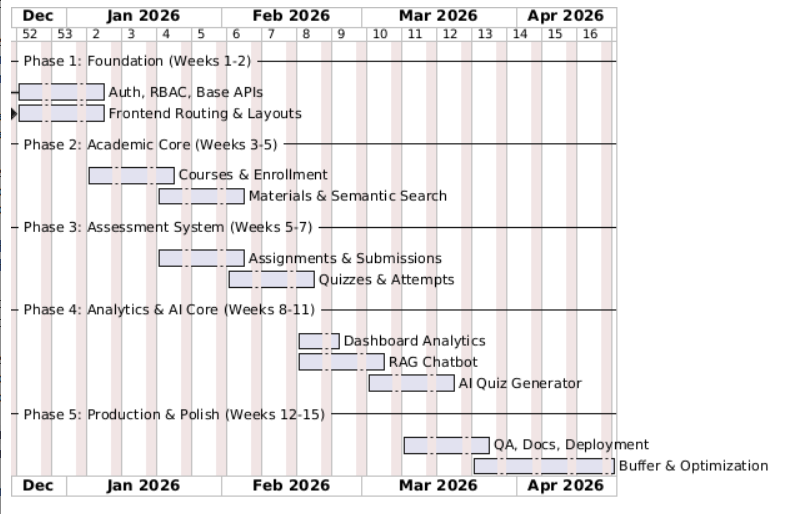
\includegraphics[width=1.1\textwidth, keepaspectratio]{system_ss/gantt.png}
\caption{Gantt Chart of the SyncAcademy Project Timeline (Weeks 1--13)}
\label{fig:gantt}
\end{figure}

\section{Applications of the Work}

SyncAcademy can be used directly with: (1) university course delivery as an intelligent replacement for static LMS platforms (2) AI-assisted self-teaching when students don't have access to private tutoring (3) formative assessment analytics enabling instructors to monitor class level topic engagement (4) academic event coordination for departments managing viva and thesis defence schedules across multiple courses and (5) research into adaptive learning systems and educational data mining, for which the tagging pipeline and Synthetic Data Lab provide a reproducible experimental foundation. Sixth, it functions as an on-demand question bank generator, allowing instructors to produce fresh, context-specific quiz questions from their own lecture materials rather than relying on generic or recycled question pools. Seventh, it supports bridge course and remedial training programs, where students can be automatically recommended foundational materials based on identified gaps in prerequisite knowledge. Eighth, it serves as a research platform for adaptive learning systems and educational data mining, for which the tag-based performance tracing pipeline and Synthetic Data Lab provide a reproducible, privacy-preserving experimental foundation. Ninth, it can be deployed in peer learning and study group scenarios, where students can collaboratively search course materials and validate each other's understanding using the AI Tutor as a neutral reference. Tenth, it offers a low-cost alternative for resource-constrained institutions, since the core AI components can run on local hardware using Ollama without expensive commercial API subscriptions.

\section{Organization of the Project}

Chapter II shows us the related literature on LMS platforms, semantic information retrieval, Retrieval-Augmented Generation, and tag-based recommendation systems etc. Chapter III refers the complete system methodology including architecture, data modelling, and algorithmic design. Chapter IV covers implementation details, results, and discussion. Chapter V addresses ethical, legal, and societal concerns. Chapter VI analyses complex engineering problems and activities. Chapter VII concludes with a summary, acknowledged limitations, and future directions.

Chapter II shows us the related literature on LMS platforms, semantic information retrieval,
Retrieval-Augmented Generation, and tag-based recommendation systems etc. Chapter III
refers the complete system methodology including architecture, data modelling, and
algorithmic design. Chapter IV covers implementation details, results, and discussion.
Chapter V addresses ethical, legal, and societal concerns. Chapter VI analyses complex
engineering problems and activities. Chapter VII concludes with a summary, acknowledged
limitations, and future directions.
%============================================================
\chapter{Related Works}
%============================================================

\section{Introduction}

This chapter shows the four technical domains underpinning SyncAcademy: learning
management systems, dense information retrieval, Retrieval-Augmented Generation, and
tag based content recommendation. Each section identifies gap of previous work that SyncAcademy’s integrated design fills and also justifies the technical choices described in Chapter III. 
\section{Learning Management Systems}

The history of learning management systems (LMS) is quite old. Early platforms like WebCT (1995) and Blackboard (1997) started the idea of delivering courses through the web in higher education. Later, in 2003, Dougiamas and Taylor introduced Moodle as an open-source alternative, and over time it became one of the most widely used LMS platforms in the world \cite{moodle}. After that, newer cloud-based platforms such as Google Classroom (2014) and Canvas made the system simpler and more integrated with everyday tools. However, even though these platforms are very popular, they still have some common limitations. As Siemens and Long pointed out \cite{siemens}, most LMS platforms mainly record activities like submissions and grades, but they do not actually understand what a student has learned. Also, they usually provide the same content to all students without considering individual performance or learning level. The Learning Analytics movement tried to solve this by analyzing LMS data, but these features are usually added later and are not part of the core system design.

\section{Semantic Information Retrieval}


Classical information retrieval methods like TF-IDF and BM25 mainly depend on keyword matching. so they most times fail when different words are used for the same idea \cite{bm25}. Later, BERT \cite{bert} showed that embeddings can understand meaning, not just exact words. After that, DPR \cite{dpr} and Sentence-BERT \cite{sbert} improved these idea by using vector similarity for better search and this inspired using all-MiniLM-L6-v2 in SyncAcademy.

Research also shows that combining dense and sparse methods works better than using only one \cite{sparse_dense}. So, SyncAcademy uses cosine similarity for meaning and also a small token overlap check to avoid wrong matches. For example, ``TCP reliability'' should not match ``reliability engineering'' just because words look similar. Another important thing is that search is limited to only the courses a student is enrolled in. This helps both privacy and getting more relevant results unlike general systems which search everything.

\section{Retrieval-Augmented Generation}

Lewis et al. \cite{rag} introduced RAG where a model uses external retrieved data along with generation and it improved performance in knowledge based tasks. Later works showed that if the model is forced to answer only from given context hallucination can be reduced a lot \cite{replug}. This is important in education because wrong answers can mislead students badly.

In SyncAcademy, the RAG Tutor try to control this using strict prompts, topic checking, and a fallback response. It also has an optional selfcheck system to verify answers. But using a smaller open-source model (llama3.1) was not easy, as it often ignored instructions at first. After multiple prompt tuning, it reached very good grounded answers. Another feature is multi query retrieval, where the system breaks a question into simpler or expanded queries. This helps to find better and more relevant materials since a single query can miss useful information sometimes.


\section{Discussion}

Table~\ref{tab:related} maps prior systems to the five feature dimensions of SyncAcademy, demonstrating that no single prior work covers all five dimensions within a unified production platform.

\begin{table}[htbp]
\caption{Comparison of SyncAcademy with Related Systems and Foundational Works}
\label{tab:related}
\centering
\small
\begin{tabularx}{\textwidth}{|X|c|c|c|c|c|}
\hline
\textbf{System / Work} & \textbf{LMS} & \textbf{Sem. Search} & \textbf{RAG Tutor} & \textbf{AI Quiz} & \textbf{Tag Rec.}\\
\hline
Moodle \cite{moodle} & $\checkmark$ & & & & \\
Google Classroom & $\checkmark$ & & & & \\
DPR \cite{dpr} & & $\checkmark$ & & & \\
RAG (Lewis et al.) \cite{rag} & & $\checkmark$ & $\checkmark$ & & \\
Tag-CF (Marinho et al.) \cite{tagging} & & & & & $\checkmark$ \\
\textbf{SyncAcademy (this work)} & $\checkmark$ & $\checkmark$ & $\checkmark$ & $\checkmark$ & $\checkmark$ \\
\hline
\end{tabularx}
\end{table}

Beyond dimensional coverage, SyncAcademy distinguishes itself through several architectural and operational characteristics that are not captured in a simple feature checklist. Unlike traditional LMS platforms that treat AI capabilities as optional add-ons, SyncAcademy embeds intelligence into its core data pipeline—materials are automatically chunked and embedded upon upload, making them immediately available for semantic search, RAG retrieval, and quiz generation without redundant processing. This design ensures consistency across all three AI subsystems, as they operate on identical vector representations of the same source content.

Another key differentiator is the evidence-based validation pipeline. While generic RAG systems may retrieve and generate without verification, SyncAcademy implements a multi-step gate: retrieved chunks must pass a relevance threshold, generated answers undergo self-evaluation, and quiz questions are explicitly traced to source sentences. This design directly addresses the hallucination problem that plagues educational applications of large language models.

Furthermore, the academic event management subsystem represents a novel contribution absent from both commercial and open-source LMS platforms. The ability to coordinate cross-course evaluations—such as joint vivas or shared project defenses—with automatic mark aggregation solves an operational problem that university departments currently handle through spreadsheets or custom scripts.

To provide a more granular comparison of operational capabilities, Table~\ref{tab:operational} evaluates SyncAcademy against existing systems across nine practical dimensions.

\begin{table}[htbp]
\caption{Operational Feature Comparison Across Educational Platforms}
\label{tab:operational}
\centering
\small
\begin{tabularx}{\textwidth}{|X|c|c|c|}
\hline
\textbf{Feature} & \textbf{Moodle} & \textbf{Google Classroom} & \textbf{SyncAcademy} \\
\hline
Role-based access with domain auto-detection & Partial (manual) & & $\checkmark$ \\
\hline
Semantic material search & & & $\checkmark$ \\
\hline
Source-grounded AI tutor & & & $\checkmark$ \\
\hline
Evidence-based quiz generation & & & $\checkmark$ \\
\hline
Tag-based performance recommendations & & & $\checkmark$ \\
\hline
Cross-course event management & & & $\checkmark$ \\
\hline
Synthetic data generation for testing & & & $\checkmark$ \\
\hline
Local LLM deployment option & & & $\checkmark$ \\
\hline
In-app notification engine (14+ event types) & Partial & Partial & $\checkmark$ \\
\hline
Teacher-to-teacher course invitations & & & $\checkmark$ \\
\hline
\end{tabularx}
\end{table}

As Table~\ref{tab:operational} shows, while Moodle offers extensive plugin-based extensibility and Google Classroom provides simplicity, neither platform natively supports the integrated AI capabilities that are central to SyncAcademy. The absence of semantic search, grounded AI tutoring, and evidence-based quiz generation from mainstream LMS platforms represents a significant gap in addressing modern engineering education needs, particularly in contexts like KUET where large class sizes and limited TA support create demand for intelligent self-study assistance.

SyncAcademy does not claim to replace Moodle's deep ecosystem of assessment plugins or Google Classroom's mature infrastructure. Rather, it demonstrates that a purpose-built system can integrate multiple AI capabilities within a coherent architecture, offering a reference implementation for future LMS designs that prioritize intelligence as a first-class concern rather than an afterthought. The Synthetic Data Lab further supports reproducibility and experimentation, enabling researchers to conduct ablation studies and benchmark alternative recommendation algorithms without exposing real student data.

Finally, the choice of locally-hostable components (Ollama, open-source embedding models) distinguishes SyncAcademy from cloud-dependent AI tutoring systems. This design prioritizes institutional data privacy and offline accessibility, which are critical requirements in many educational settings where student data cannot be transmitted to third-party APIs.
%============================================================
\chapter{Methodology}
%============================================================

\section{Introduction}

Here, the entire methodology of SyncAcademy is introduced: the overall system architecture, the entire database design, and the specific algorithm design of each subsystem such as authentication, course management, the announcement and assignment system, academic events, semantic search, the RAG AI Tutor, the AI quiz generation, and the tag-based adaptive recommendation system.

\section{Overall System Architecture}

SyncAcademy is a web architecture with three layers and an AI services layer. The presentation level is a single-page React 18 application. The application layer is a stateless 25-route-module Node.js / Express 4 API server. The data layer is a MongoDB Atlas database connected with Mongoose 9. The AI services layer, which sits adjacent to the application layer, includes an Ollama local LLM server (running the \texttt{llama3.1} model) for text generation and quiz creation, the Hugging Face Inference API (\texttt{BAAI/bge-small-en-v1.5} and \texttt{all-MiniLM-L6-v2}) for sentence embedding with an OpenAI-compatible fallback, and Cloudinary as a CDN service to store static content.

\begin{figure}[htbp]
\centering
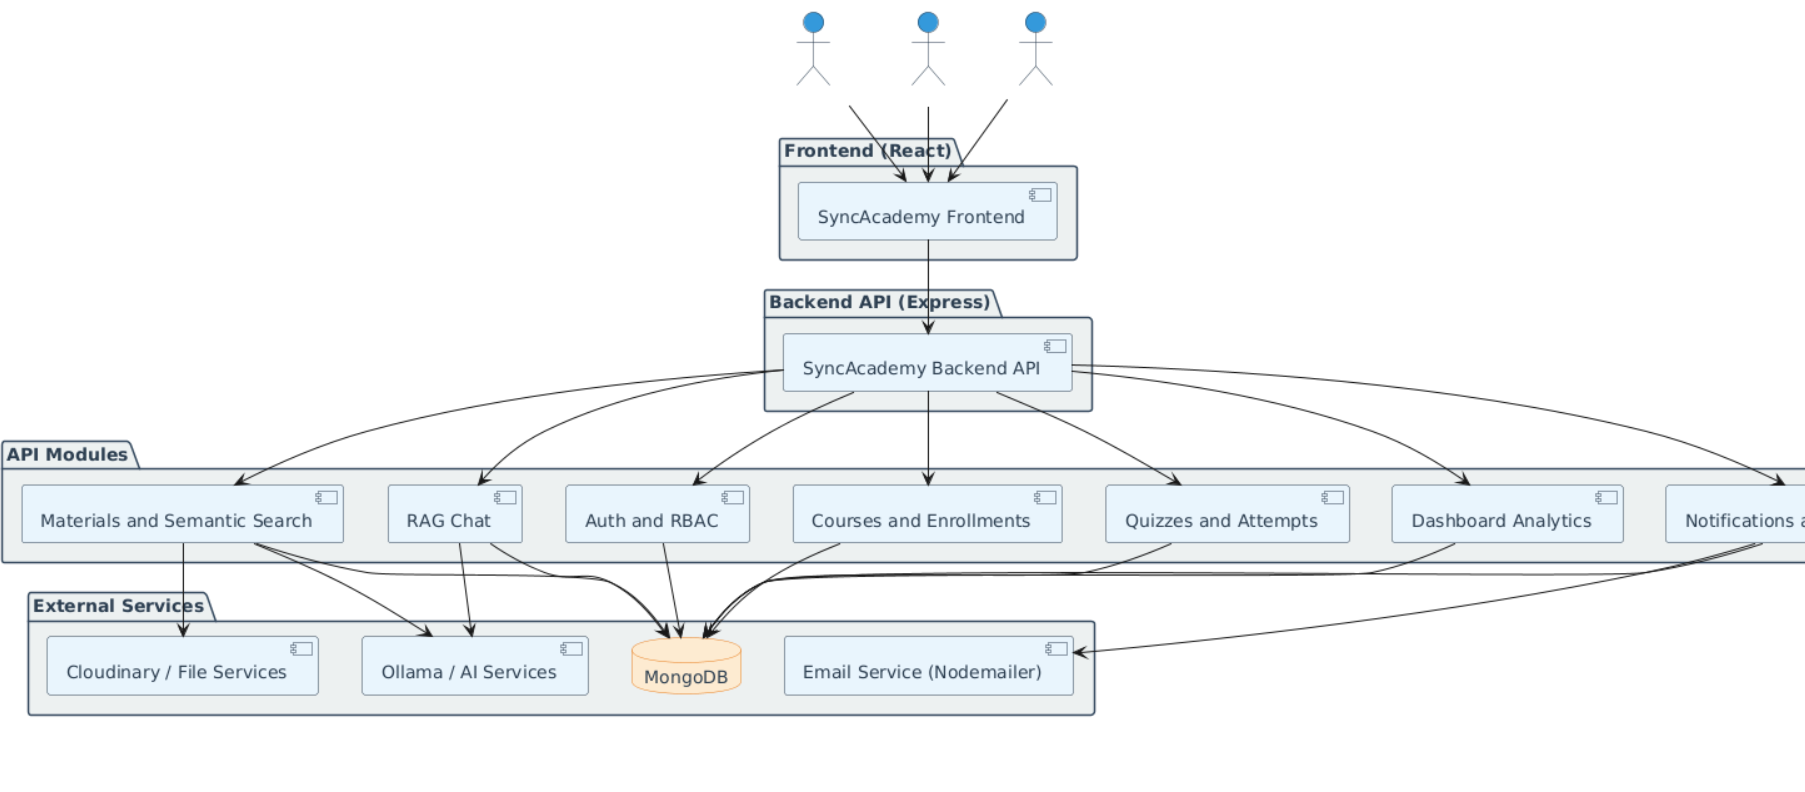
\includegraphics[angle=90, width=0.9\textwidth, height=0.8\textheight]{system_ss/system_arch.png}
\caption{Overall System Architecture of SyncAcademy}
\label{fig:architecture}
\end{figure}

\begin{figure}[htbp]
\centering
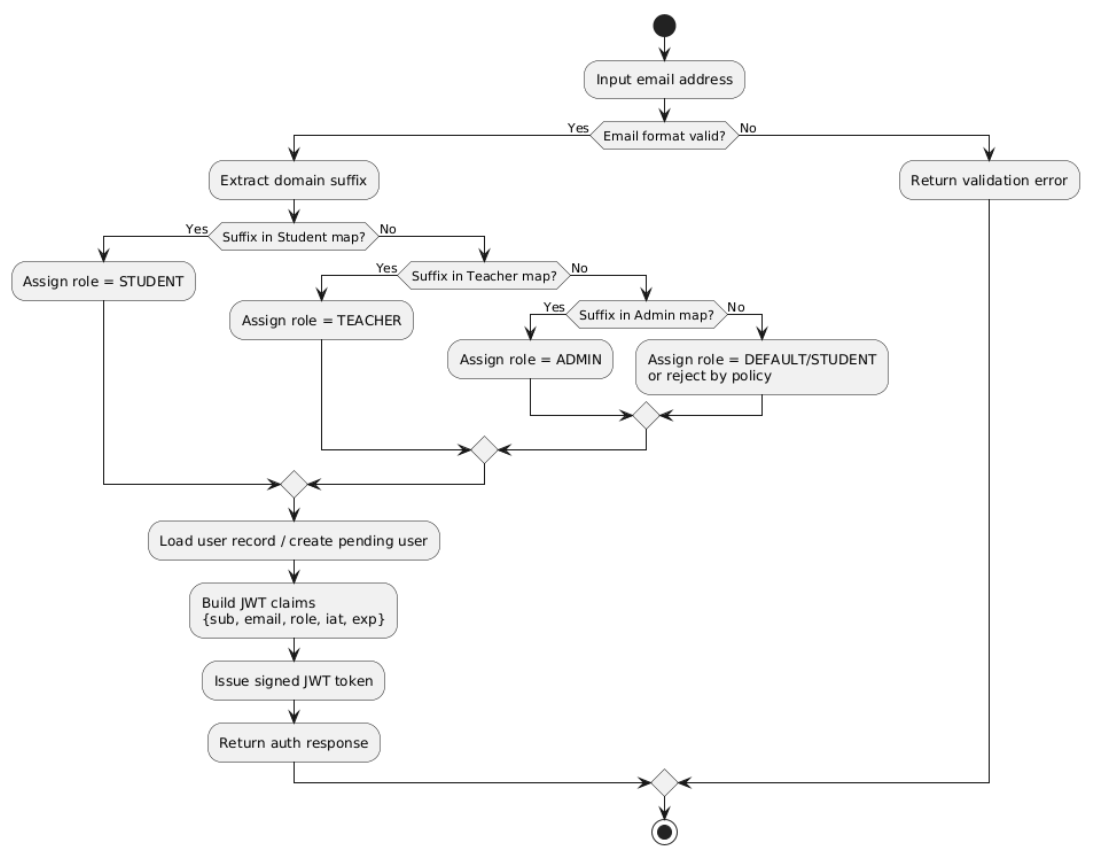
\includegraphics[width=\textwidth,height=0.82\textheight,keepaspectratio]{system_ss/email_domain.png}
\caption{KUET Email-Based Automatic Role Detection at Registration}
\label{fig:role_detect}
\end{figure}
\section{Data Model and Schema Design}

SyncAcademy's MongoDB database comprises twenty one collections. Table~\ref{tab:models} summarises each collection with its primary fields and indexing strategy.

\begin{table}[htbp]
\caption{Primary MongoDB Collections, Key Fields, and Index Strategy}
\label{tab:models}
\centering
\small
\begin{tabularx}{\textwidth}{|l|X|}
\hline
\textbf{Collection} & \textbf{Key Fields and Index Notes} \\
\hline
\textbf{User} & name, email (unique), password (bcrypt), role (student/teacher/admin), idNumber (7-digit, sparse-unique), avatar (Cloudinary URL), isVerified, otp, otpExpiry \\
\textbf{Course} & courseNo (unique), courseTitle, courseCode (8-char hex, unique, auto-generated), description, department, semester, createdBy, coTeachers \\
\textbf{Enrollment} & student (ref User), course (ref Course), enrolledAt, status (active/dropped); compound unique index (student, course) \\
\textbf{Material} & courseTitle, courseNo, type, fileUrl (Cloudinary signed URL), originalFileName, textContent, topicTags (array: topicId, subtopicId, confidence, source); index on courseNo \\
\textbf{MaterialChunk} & materialId (ref Material), chunkText, embedding (dense float array); used for vector retrieval \\
\textbf{TopicTaxonomy} & courseNo, topics (topicId, name, subtopics, aliases) \\
\textbf{TopicAlias} & topicId, aliases (array of strings) \\
\textbf{Announcement} & course, author, title, content, isPinned, attachments (fileName, fileUrl, fileType), links, comments (subdoc: user, text, replies, editedAt); index (course, isPinned, createdAt) \\
\textbf{Assignment} & course, createdBy, title, description, dueDate, totalMarks, attachments, allowLateSubmission, isResultPublished, resultSheetUrl; index (course, createdAt) \\
\textbf{Submission} & assignment, student, fileUrl, fileName, textContent, submittedAt, isLate, grade, feedback, gradedBy, evaluatedFileUrl, showEvaluatedToStudent; unique (assignment, student) \\
\textbf{Quiz} & course, createdBy, title, questions (MCQ: questionText, 4 options, correctAnswer, explanation, difficulty, sourceChunk, topicTags), isPublished, timeLimit, scheduledAt, availableUntil \\
\textbf{QuizAttempt} & quiz, student, answers, score, percentage, timeTaken; unique (quiz, student) \\
\textbf{Discussion} & course, author, title, content, attachments, tags, views, replies (user, content, votes \{value:+1/-1\}, isAccepted, subReplies) \\
\textbf{Notification} & recipient (indexed), type (14-value enum), title, message, link, isRead, metadata; index (recipient, isRead, createdAt) \\
\textbf{Event} & title, type (central\_viva/presentation/thesis\_defense/project\_show), courses [\{course, teacher\}], eventDate, venue, registrationCode (unique 8-char hex) \\
\textbf{EventRegistration} & event, student \\
\textbf{EventMark} & event, course, student, teacher, mark \\
\textbf{CourseInvitation} & from (teacher), to (teacher), course, message, status (pending/accepted/declined); unique (from, to, course) \\
\textbf{ChatSession} & user, messages (role, content, ragMetadata, sources) \\
\textbf{Feedback} & student, message, response, isResolved; auto-cleaned by node-cron job \\
\hline
\end{tabularx}
\end{table}

\begin{figure}[p]
\centering
\includegraphics[width=1.00\textwidth, keepaspectratio]{system_ss/ER (4).png}
\caption{Entity-Relationship Diagram }
\label{fig:er1}


\end{figure}


\section{Problem Design and Analysis}

\subsection{Authentication and Role Detection}

At registration, the \texttt{detectRoleFromEmail()} utility extracts the email domain suffix and maps it to a role: \texttt{@stud.kuet.ac.bd} $\rightarrow$ student, \texttt{@kuet.ac.bd} (excluding student subdomain) $\rightarrow$ teacher, \texttt{@admin.kuet.ac.bd} $\rightarrow$ admin. A six-digit OTP is generated via \texttt{crypto.randomInt}, stored with a 10-minute expiry, and sent via Nodemailer; the account remains \texttt{isVerified: false} until verified. On login, a JWT is issued containing the user ID and role claim. All protected routes validate the token via the \texttt{protect} middleware and, where applicable, gate access by role via \texttt{authorizeRoles()}.

\subsection{Course Enrollment System}

At the time of creation, each course is given a unique eight-character hexadecimal course code via \texttt{crypto.randomBytes(4).toString('hex').toUpperCase()}. Courses may also be accessed through teacher-to-teacher course invitations: a teacher sends an invitation to another teacher, who can either accept or refuse it. If accepted, the accepting teacher is added to the \texttt{coTeachers} array. For students, the Enrollment document is a table of the student--course pair using a distinctive compound index. The enrollment scope applies to all student-facing endpoints (such as material feed, semantic search, announcement stream, assignment list, quiz list, etc.), enforcing course access boundaries.

\subsection{Announcement Stream}

The announcement model accepts textual content, several files with type classification (image/document) and links. Nested comments embrace two layers: top-level comments and sub-replies, each having edit timestamps. A compound MongoDB index on (course, isPinned: -1, createdAt: -1) guarantees that when showing announcements, pinned announcements are returned first. When an announcement is created, the helper method \texttt{notifyEnrolledStudents()} notifies all active enrolled students by sending them an announcement notification.

\subsection{Assignment and Grading System}

Educators generate tasks that have due dates, marks per task, and optional attachments of reference files. The system allows file uploading (Cloudinary upload) and free response. Late submission is automatically detected: \texttt{isLate = submittedAt > assignment.dueDate}. Teachers mark submissions using a numerical mark and written comments. A teacher-posted consolidated PDF result sheet is stored in the field \texttt{resultSheetUrl}, and can be disclosed to students using \texttt{showEvaluatedToStudent}. When grading, an ``assignment graded'' notification is dispatched to the student. Assignment topic tags are optionally set by the teacher at creation time; these feed directly into the tag-based recommendation pipeline.

\subsection{AI Quiz Generator}

The quiz generator service retrieves all MaterialChunk documents in the target course, picks a random sample of them (biased towards longer chunks, up to $N+2$ chunks in total for $N$ target questions), and asks Ollama to generate one MCQ at a time with a structured JSON template. All generated questions are grounding-validated: tokens of key-terms of the \texttt{questionText} must be present verbatim in the source \texttt{chunkText} at a minimum match ratio. Questions which do not pass this test are rejected, so that hallucinated questions are not given to the teacher review interface. The teacher can then revise, delete, or re-sequence questions prior to publication. Each generated question carries a \texttt{topicTags} field derived from the source chunk's parent material, which feeds the tag-based recommendation system when a student attempts the quiz.

\subsection{Academic Event Management}

The event system supports four types: Central Viva, Presentation, Thesis Defence, and Project Show. An event is created by a teacher; it has a date, a venue, and a list of courses involved, each with a marking teacher associated with it. The assigned teachers are notified of the event invite via a notification of event invite. Students enroll by use of a one-time eight-character registration code. The designated teacher adds individual marks to each student of his/her course. The mark sheet is consolidated and downloadable to the event creator. The status of the event (upcoming/completed) is calculated dynamically based on the current timestamp in comparison with the event date.

\subsection{Discussion Forum}

The discussion module is a course-wide question-and-answer board. Students ask questions with optional file attachments. Any registered student or teacher is allowed to reply; replies have sub-replies (2 levels of nesting), can be upvoted/downvoted with a schema of [value: +1/--1], and there is a flag \texttt{isAccepted} that the question author or a teacher can set. Sorted feed queries are efficiently supported through compound indexes on (course, createdAt) and on view count.

\subsection{Semantic Search Algorithm}

\begin{figure}[htbp]
\centering
\includegraphics[width=\textwidth, height=0.82\textheight, keepaspectratio]{system_ss/semantic_search.png}
\caption{Complete Pipeline of Semantic Search}
\label{fig:semantic_search}
\end{figure}

Suppose there is a student query, denoted by $q$. The search pipeline is as follows:

\begin{enumerate}
\item \textbf{Query validation}: The query is verified with the minimum character length (3), minimum number of meaningful words (2), maximum non-alphanumeric ratio (0.45), and minimum number of unique characters (3). Queries with malformations or gibberish are automatically rejected.

\item \textbf{Embedding and Candidate Loading}: The query is embedded to get the query representation vector, denoted by $\vec{q} \in \mathbb{R}^d$. The embedding arrays of all \texttt{MaterialChunk} documents of the active enrolled courses of the student are loaded.

\item \textbf{Hybrid Scoring}: The cosine similarity and token overlap ratio of each chunk $c_i$ are calculated:
\begin{equation}
  \text{cos}(i) = \frac{\vec{c}_i \cdot \vec{q}}{\|\vec{c}_i\| \|\vec{q}\|}
  \qquad
  \text{overlap}(i) = \frac{|\text{tokens}(q) \cap \text{tokens}(c_i)|}{|\text{tokens}(q)|}
\tag{3.1}
\end{equation}
A chunk is retained if both $\text{cos}(i) \geq \tau_s$ and $\text{overlap}(i) \geq \tau_o$, where $\tau_s = 0.40$ and $\tau_o = 0.08$ (for short queries: $\tau_o = 0.34$). The cosine similarity of retained chunks serves as the hybrid score.

\item \textbf{Grouping and Ranking}: The 50 highest-scoring chunks are clustered by parent \texttt{Material}; the score of a material is the highest score among its chunks. Sorting is descending; the top 20 are returned, each having up to five snippets of matching excerpts.
\end{enumerate}

The lexical overlap gate is the most important differentiator from pure dense retrieval. Without it, the embedding model's general semantic space can produce false-positive matches where a query about TCP networking retrieves slides about Bayesian networks purely because both concern ``network'' concepts. The gate requires genuine word-level intersection, eliminating this class of misleading results. Table~\ref{tab:search_thresholds} summarises the threshold values and their effect on precision and recall.

\begin{table}[htbp]
\caption{Semantic Search Threshold Configuration and Effect}
\label{tab:search_thresholds}
\centering
\small
\begin{tabularx}{\textwidth}{|l|c|X|}
\hline
\textbf{Parameter} & \textbf{Value} & \textbf{Effect} \\
\hline
$\tau_s$ (cosine threshold) & 0.40 & Minimum semantic similarity; set empirically to balance precision and recall \\
$\tau_o$ (overlap, long query) & 0.08 & Minimum token overlap for standard queries ($\geq$4 tokens) \\
$\tau_o$ (overlap, short query) & 0.34 & Stricter overlap for queries with fewer than 4 tokens to avoid false positives \\
Top-N pre-grouping limit & 50 & Maximum chunks scored before material grouping \\
Top-K materials returned & 20 & Final ranked material results per search \\
Snippets per material & 5 & Number of matching text excerpts shown per result \\
\hline
\end{tabularx}
\end{table}

\subsection{RAG AI Tutor Pipeline}

The RAG pipeline consists of five stages, illustrated in Figures~\ref{fig:rag1} and~\ref{fig:rag2}:

\textbf{Stage 1 : Query Analysis}. The \texttt{queryAnalyzer} classifies the query as simple, moderate, or complex based on entity count, question type, and token length. It also generates semantically expanded sub-queries for multi-query retrieval. A simple factual question (``What is a semaphore?'') is classified as simple and retrieves two sub-queries. A comparison or multi-part question (``Compare mutual exclusion and synchronisation in operating systems'') is classified as complex and retrieves up to five sub-queries.

\textbf{Stage 2 : Adaptive Multi-Query Retrieval}. Based on the complexity class, the retriever selects parameters from Table~\ref{tab:retrieval}. Each sub-query is embedded and scored against all enrolled-course chunks. Results are merged by keeping the maximum score per deduplicated chunk (deduplication key: first 80 characters of chunk text).

\begin{table}[htbp]
\caption{Adaptive Retrieval Parameters by Query Complexity Class}
\label{tab:retrieval}
\centering
\small
\begin{tabular}{|l|c|c|c|}
\hline
\textbf{Complexity} & \textbf{Sub-queries} & \textbf{Top-K chunks} & \textbf{Min sim. threshold} \\
\hline
Simple & 2 & 3 & 0.42 \\
Moderate & 3 & 5 & 0.40 \\
Complex & 5 & 8 & 0.38 \\
\hline
\end{tabular}
\end{table}

\textbf{Stage 3 : Topic Relevance Gate}. Domain-specific noun tokens (length $\geq 5$, not in a 60-word stop list) are extracted from the query. If the fraction of these tokens appearing verbatim in the combined retrieved chunk texts is below a complexity-specific minimum ratio, the query is considered out-of-scope and the no-information fallback is returned without invoking the LLM. This gate prevents the LLM from generating a plausible-sounding but hallucinated answer for queries that happen to retrieve marginally relevant chunks.

\textbf{Stage 4 : Context-Constrained Answer Generation}. A strict system prompt is prepended that: (1) instructs the model to use only the provided context; (2) forbids training-knowledge use by name; (3) specifies an exact fallback phrase for insufficient context; (4) imposes a three-sentence maximum. The response UI includes citations to the source document, enabling the student to follow up on the original material.

\textbf{Stage 5 : Self-Evaluation (Optional)}. If \texttt{RAG\_ENABLE\_SELF\_EVAL=true}, the \texttt{selfEvaluator} makes a second Ollama call to evaluate the draft response on faithfulness $\in [0,1]$ and coverage $\in [0,1]$. If either is below the configurable threshold (\texttt{RAG\_SELF\_EVAL\_THRESHOLD}, default 0.5), the retrieval is broadened by one difficulty level and the draft answer is regenerated (at most \texttt{RAG\_MAX\_RETRIES} times).

\begin{figure}[p]
\centering
\includegraphics[width=0.72\textwidth, keepaspectratio]{system_ss/seq1.png}
\caption{Five-Stage RAG AI Tutor Request-Response Sequence Diagram - Part 1}
\label{fig:rag1}

\includegraphics[width=0.72\textwidth, keepaspectratio]{system_ss/seq2.png}
\caption{Five-Stage RAG AI Tutor Request-Response Sequence Diagram - Part 2}
\label{fig:rag2}
\end{figure}

The multi-session chat history is preserved in a ChatSession document and displayed in a collapsible sidebar, allowing students to resume prior tutoring conversations across browser sessions. Each message in the history carries \texttt{ragMetadata} (sources, confidence, stage reached) and a \texttt{sources} array of cited materials, giving teachers and administrators full auditability of what context was used to generate each answer.

\subsection{Tag-Based Adaptive Recommendation System}

The recommendation engine operates on three inputs: the student's quiz attempt history (\texttt{QuizAttempt} documents), the student's assignment submission history (\texttt{Submission} documents with graded marks), and the topic tag sets on all materials of the student's enrolled courses.

\subsubsection{Per-Topic Performance Score}

For each topic $t$ in the course taxonomy, a per-student performance score $p_{s,t} \in [0,1]$ is computed by aggregating normalised scores from quiz questions and assignment submissions tagged with $t$:
\begin{equation}
  p_{s,t} = \frac{\sum_{i \in \mathcal{Q}_{s,t}} w_i \cdot q_i + \sum_{j \in \mathcal{A}_{s,t}} w_j \cdot a_j}{\sum_{i \in \mathcal{Q}_{s,t}} w_i + \sum_{j \in \mathcal{A}_{s,t}} w_j}
\end{equation}
where $\mathcal{Q}_{s,t}$ is the set of quiz questions tagged with topic $t$ that student $s$ has answered, $q_i = 1$ if the answer was correct and 0 otherwise, $\mathcal{A}_{s,t}$ is the set of tagged assignment submissions, $a_j = \text{grade}/\text{totalMarks}$, and $w_i$, $w_j$ are recency weights that decay exponentially with time so that recent interactions are more influential than older ones. If no interaction has been recorded for topic $t$, a neutral prior of $p_{s,t} = 0.5$ is used.

\subsubsection{Recommendation Ranking}

Let $T_j$ be the set of topic tags assigned to material $M_j$ and $p_{s,t}$ the per-topic performance score for student $s$ on topic $t$. The recommendation rank score for material $M_j$ is:
\begin{equation}
  \text{rank}(M_j) = \frac{1}{|T_j|} \sum_{t \in T_j} (1 - p_{s,t})
\end{equation}
Materials are ordered by rank score in descending order (highest inverse performance first), ensuring that materials covering topics where the student has performed least well are surfaced first. If no topic tags are associated with any material in the course, a fallback ordering by recency (most recently uploaded materials first) is applied.

\subsubsection{Recommendation Explainability}

Each recommended material is accompanied by a tag-level explanation: a breakdown showing which topic tags contributed to its rank, the student's performance score on each tag, and the confidence of the material's assignment to those tags. This per-material explainability makes the recommendation actionable --- a student who sees that a recommended slide deck covers ``Memory Paging'' at which they scored 0.32 can immediately understand why the system is pointing them there, and a teacher reviewing the recommendation panel can audit the logic at the topic level.

\begin{figure}[htbp]
\centering
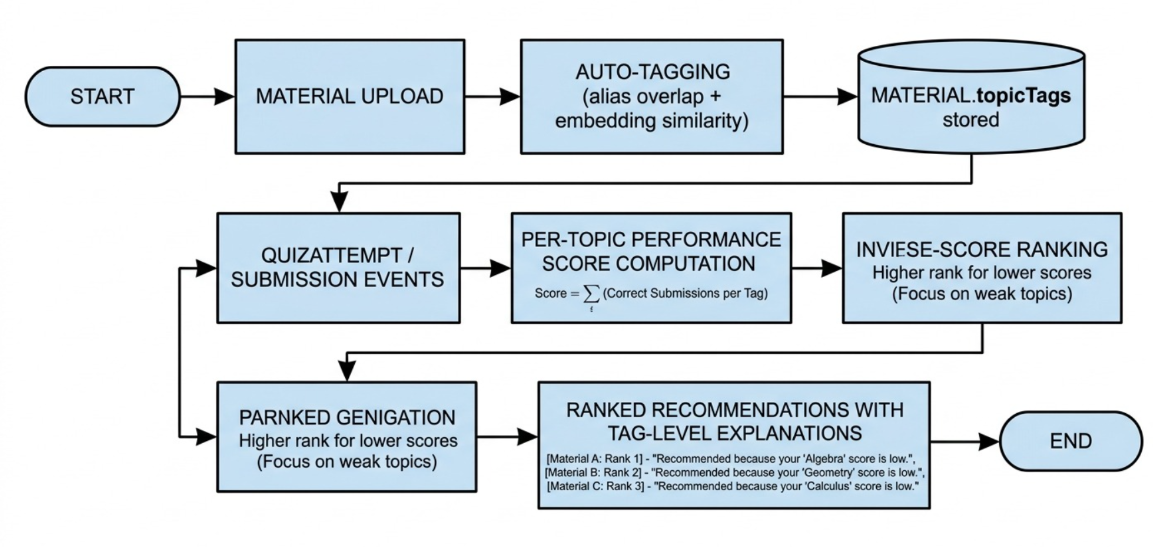
\includegraphics[width=0.93\textwidth, keepaspectratio]{system_ss/recomm_pipeline.png}
\caption{Tag-Based Adaptive Material Recommendation Pipeline}
\label{fig:rec_pipeline}
\end{figure}
\section{Overall System Framework and Flowcharts}

\begin{figure}[htbp]
\centering
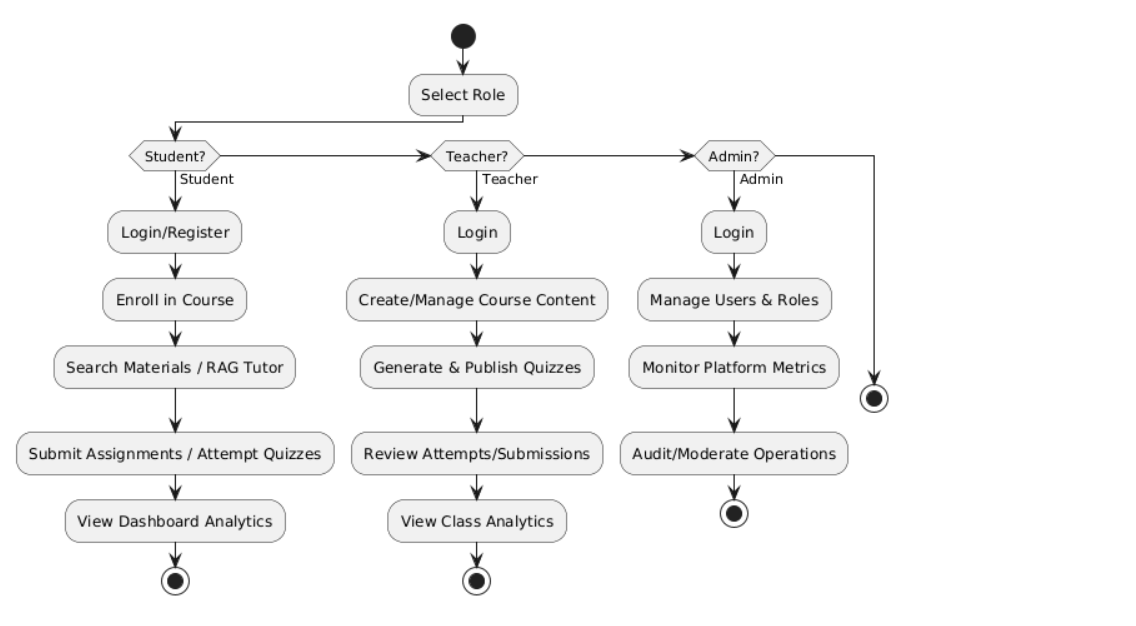
\includegraphics[width=0.93\textwidth]{system_ss/activity.png}
\caption{Activity Diagram for the Student Role Workflow}
\label{fig:activity}
\end{figure}

\begin{figure}[htbp]
\centering
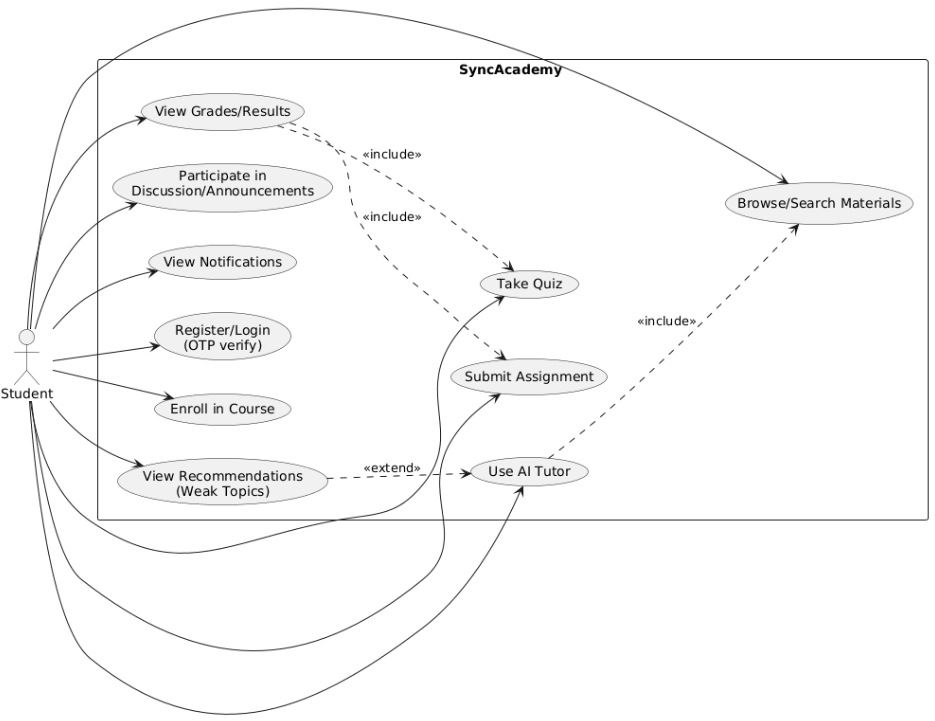
\includegraphics[width=0.93\textwidth]{system_ss/student_use.png}
\caption{Use Case Diagram for Student Workflows}
\label{fig:student_use}
\end{figure}

\begin{figure}[htbp]
\centering
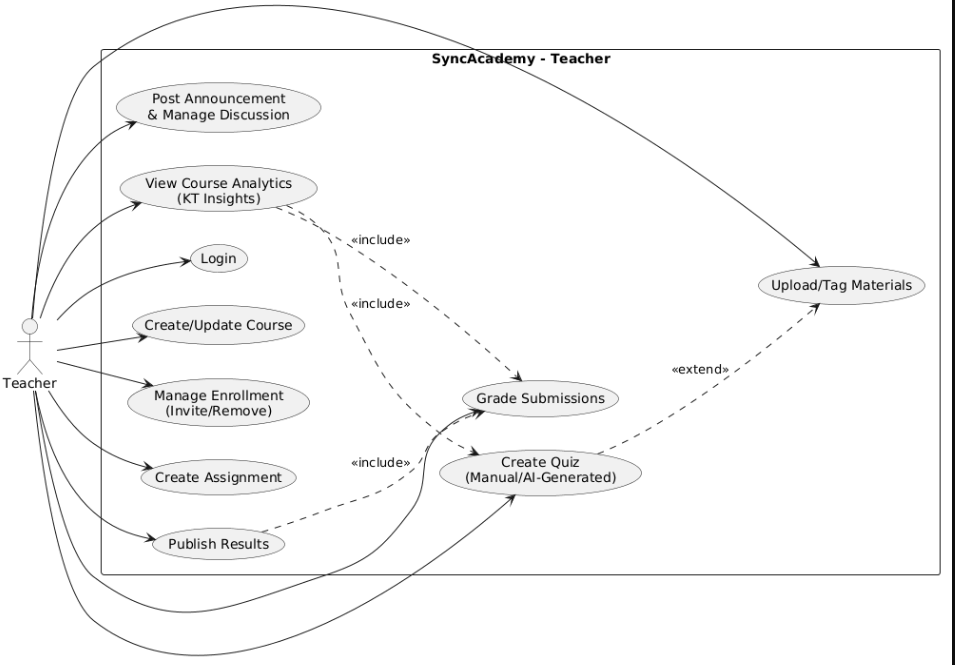
\includegraphics[width=0.93\textwidth]{system_ss/teacher_use.png}
\caption{Use Case Diagram for Teacher Workflows}
\label{fig:teacher_use}
\end{figure}

\begin{figure}[htbp]
\centering
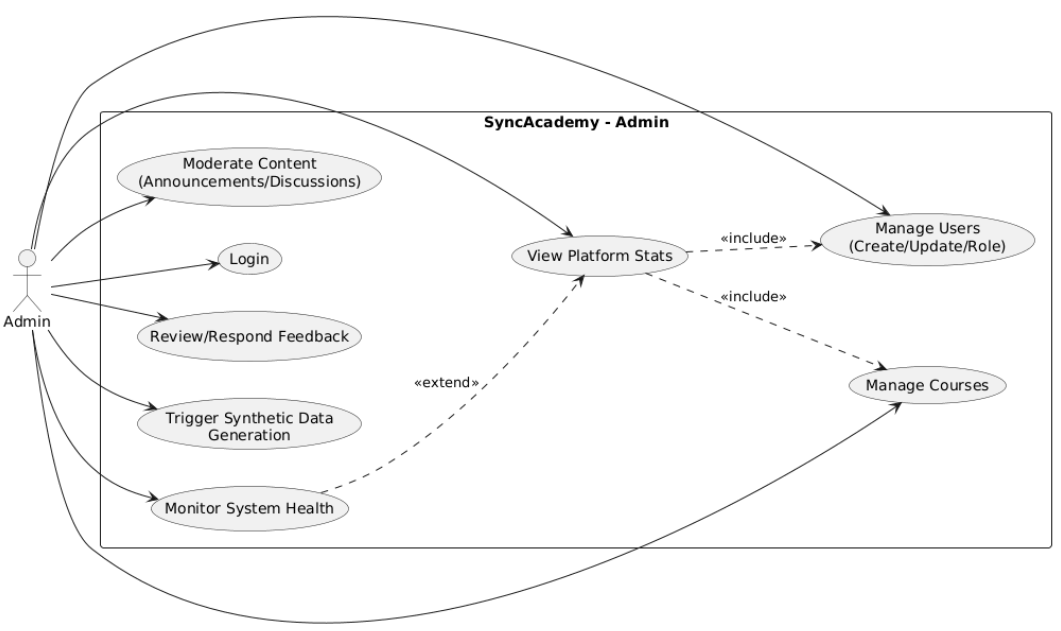
\includegraphics[width=0.93\textwidth]{system_ss/admin_use.png}
\caption{Use Case Diagram for Admin Workflows}
\label{fig:admin_use}
\end{figure}

\begin{figure}[htbp]
\centering
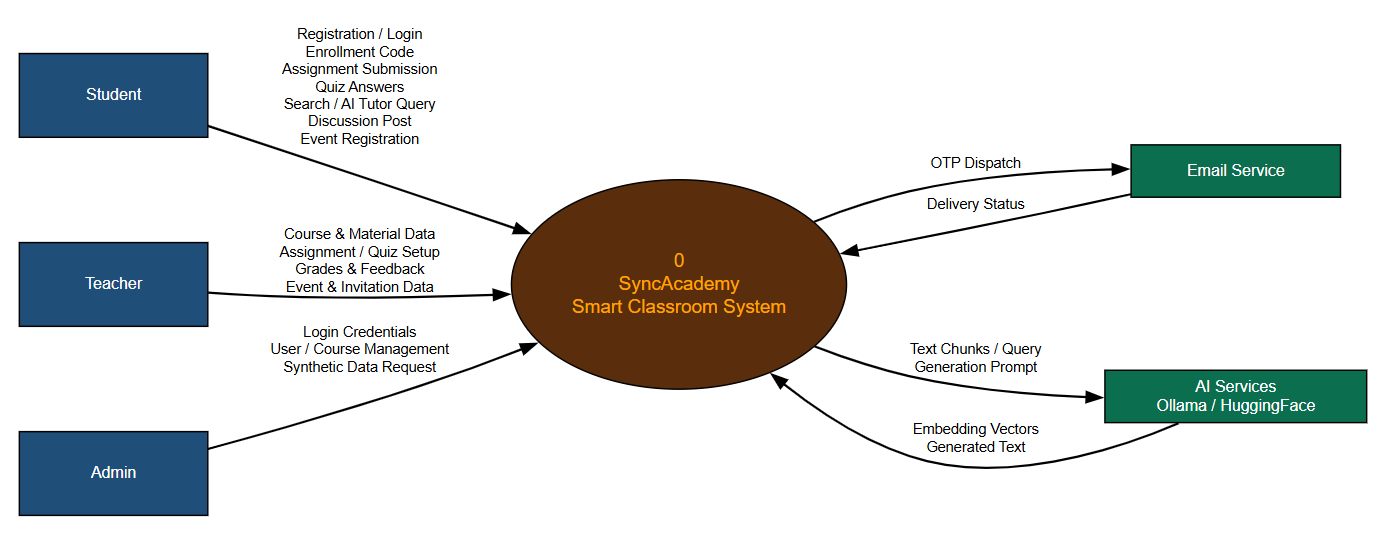
\includegraphics[width=0.93\textwidth]{system_ss/level0.png}
\caption{Level-0 Data Flow Diagram of SyncAcademy}
\label{fig:dfd_level0}
\end{figure}

\begin{figure}[htbp]
\centering
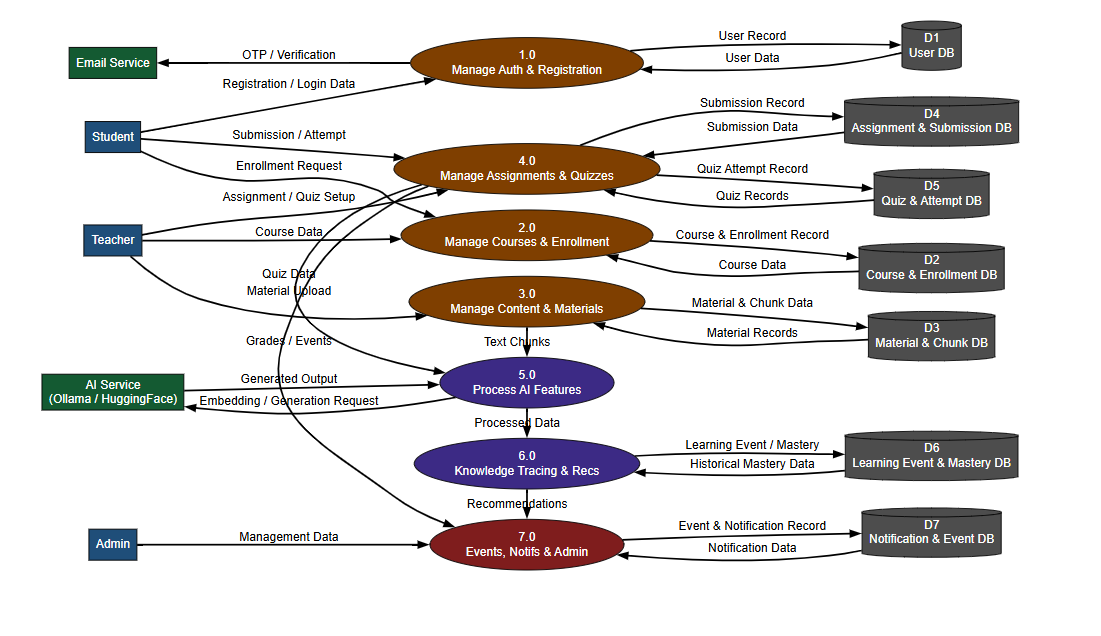
\includegraphics[width=\textwidth,height=0.95\textheight,keepaspectratio]{system_ss/level1.png}
\caption{Level-1 Data Flow Diagram of SyncAcademy}
\label{fig:dfd_level1}
\end{figure}

\section{Conclusion}

This chapter has presented the complete methodology of SyncAcademy: the three-tier architecture, the twenty MongoDB collections with their indexing strategies, and the detailed algorithmic design of authentication, enrollment, announcement, assignment, event, semantic search, RAG AI Tutor, quiz generation, material auto-tagging, and tag-based adaptive recommendation subsystems. The following chapter describes the implementation in practice and presents experimental results.

%============================================================
\chapter{Implementation, Results and Discussions}
%============================================================

\section{Introduction}

This chapter describes the technology stack and implementation details of each major subsystem, presents qualitative results from the deployed application, and reports quantitative evaluation results for the AI components.

\section{Experimental Setup}

\subsection{Technology Stack}

Table~\ref{tab:stack} lists the complete technology stack deployed in SyncAcademy.

\begin{table}[htbp]
\caption{SyncAcademy Complete Technology Stack}
\label{tab:stack}
\centering
\small
\begin{tabularx}{\textwidth}{|l|X|}
\hline
\textbf{Layer} & \textbf{Technology and Version} \\
\hline
Runtime & Node.js 18 LTS \\
API Framework & Express 4.19 \\
ODM / Database & Mongoose 9.0 + MongoDB Atlas \\
Authentication & jsonwebtoken 9, bcryptjs 3 (cost factor 10) \\
File Upload & Multer 2 (50 MB limit, PDF/DOCX/PPTX only), Cloudinary SDK 2 \\
Email / OTP & Nodemailer 6, node-cron 4 (auto-cleanup resolved feedbacks) \\
Text Extraction & pdf-parse 2 (PDF), mammoth 1 (DOCX), officeparser 5 (PPTX) \\
LLM Inference & Ollama HTTP API with \texttt{llama3.1} model (local deployment) \\
Sentence Embeddings & HuggingFace Inference API (\texttt{all-MiniLM-L6-v2}); OpenAI fallback \\
Client-side PDF & pdfjs-dist 5 (file preview in browser), jsPDF 4 (result sheet generation) \\
Frontend & React 18, Material UI 5, React Router 6, Axios 1, react-hot-toast 2 \\
Deployment & Render (backend \& frontend), MongoDB Atlas (database) \\
\hline
\end{tabularx}
\end{table}

\vspace{10cm}

\subsection{Evaluation Metrics}

Table~\ref{tab:metrics} lists the evaluation metrics and targets for each AI subsystem.

\begin{table}[htbp]
\caption{Evaluation Metrics and Targets for AI Subsystems}
\label{tab:metrics}
\centering
\begin{tabular}{|l|l|c|}
\hline
\textbf{Subsystem} & \textbf{Metric} & \textbf{Target} \\
\hline
Semantic Search & Precision@5 & $\geq 0.70$ \\
Semantic Search & nDCG@10 & $\geq 0.65$ \\
RAG AI Tutor & Grounded Answer Rate & $\geq 0.85$ \\
RAG AI Tutor & Fallback Trigger Rate (off-topic queries) & $\geq 0.90$ \\
AI Quiz Generator & Grounding Pass Rate & $\geq 0.80$ \\
Tag Recommendation & Mean Reciprocal Rank (MRR) & $\geq 0.60$ \\
Tag Recommendation & Relevance Precision@3 & $\geq 0.65$ \\
\hline
\end{tabular}
\end{table}

\subsection{Dataset}

For semantic search and RAG evaluation, a test set of 60 queries was manually annotated, derived from the content of ten uploaded lecture slide decks, with relevance judgements agreed between the two authors. For the tag-based recommendation evaluation, 30 simulated student performance profiles were generated using the Synthetic Data Lab, each with varied quiz and assignment performance distributions across five topic areas, and the top-3 recommendations were compared against a human-authored ideal ranking for each profile.

\vspace{20cm}

\section{Implementation and Results}

\subsection{Qualitative Results}

\begin{figure}[H]
\centering
\begin{minipage}[t]{0.48\textwidth}
  \centering
  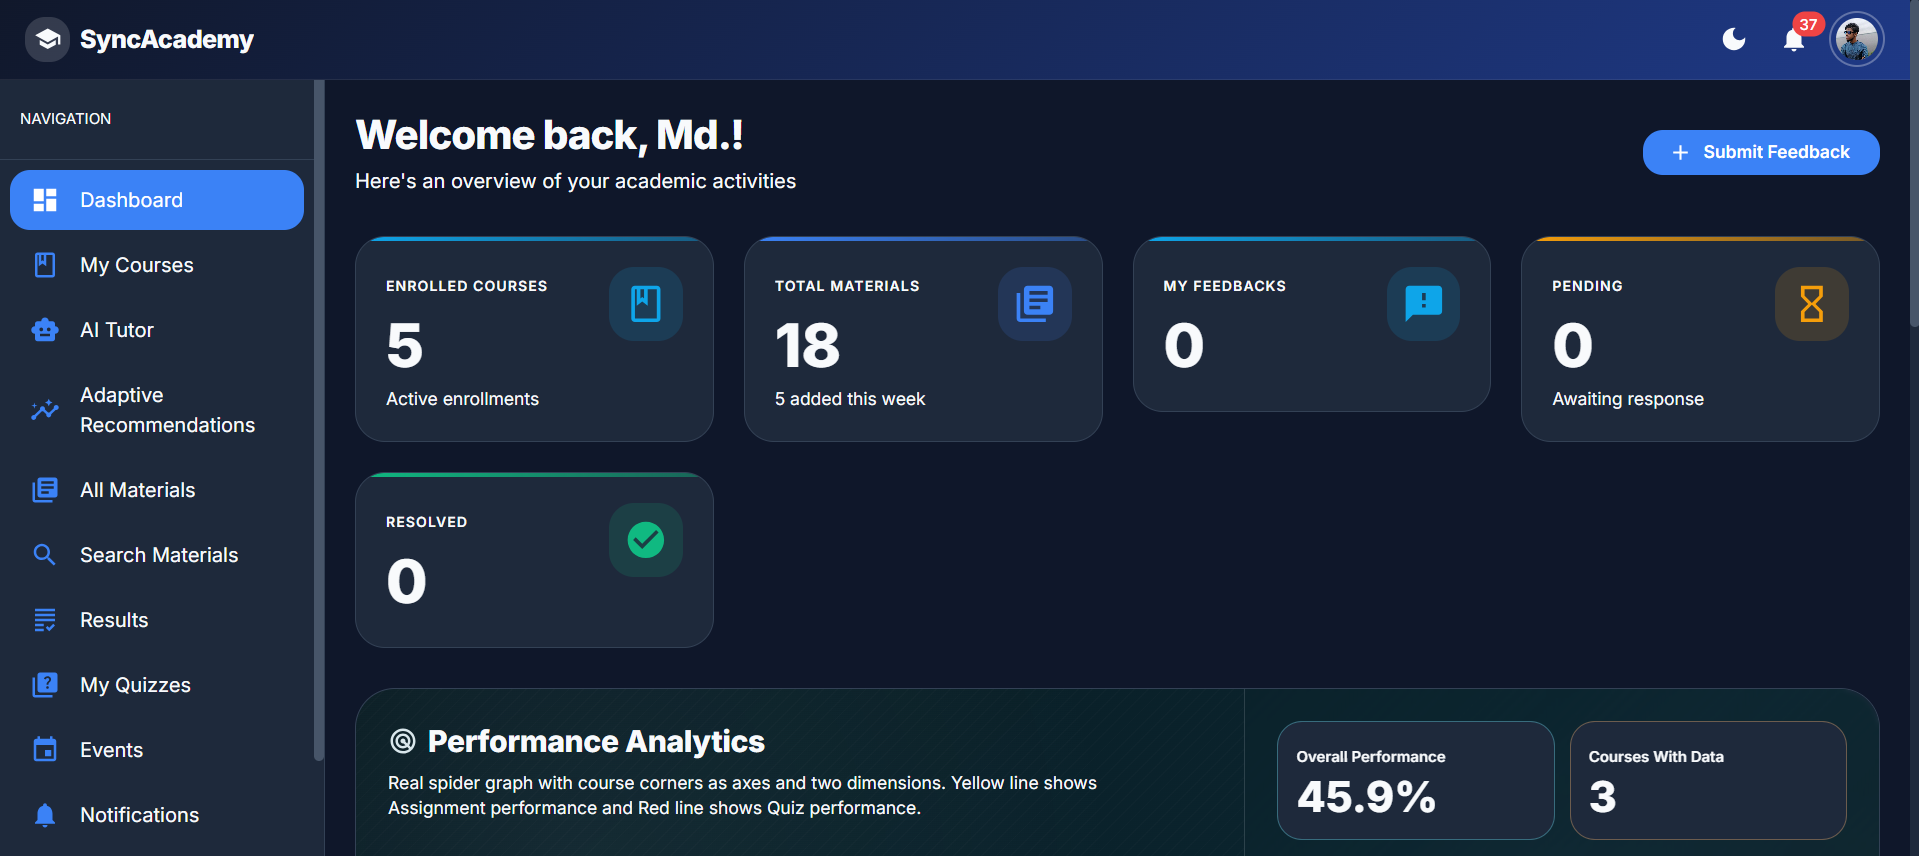
\includegraphics[width=\textwidth,height=0.31\textheight,keepaspectratio]{system_ss/student_dash.png}
  \captionof{figure}{Student Role Dashboard}
  \label{fig:ss_student_dash}
\end{minipage}\hfill
\begin{minipage}[t]{0.48\textwidth}
  \centering
  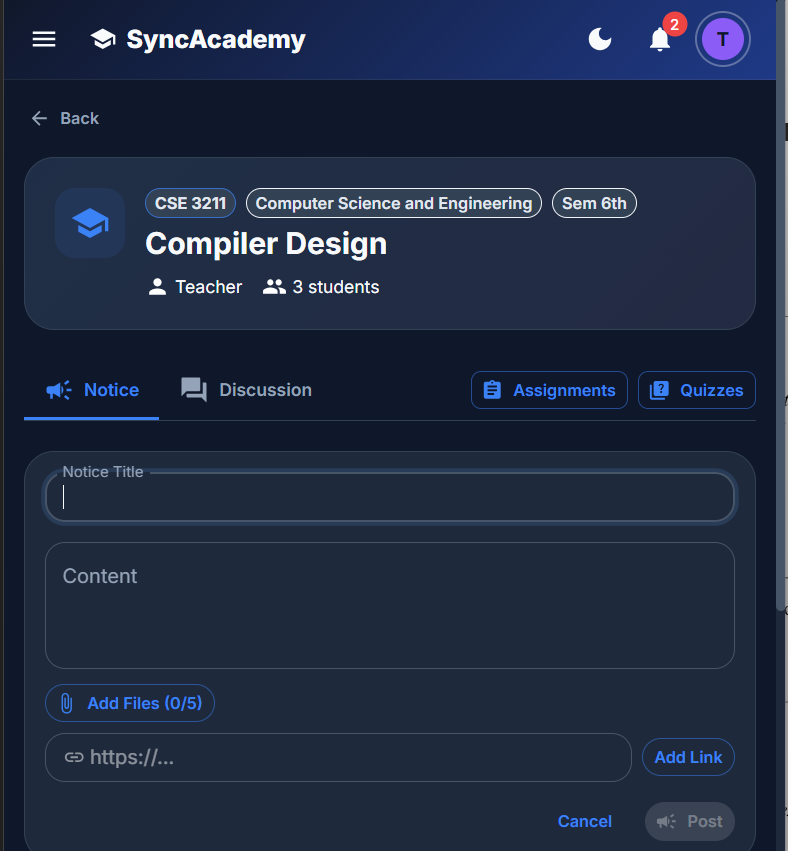
\includegraphics[width=\textwidth,height=0.31\textheight,keepaspectratio]{system_ss/announce.png}
  \captionof{figure}{Course Announcement Stream}
  \label{fig:ss_stream}
\end{minipage}
\end{figure}
\begin{figure}[H]
\centering
\begin{minipage}[t]{0.48\textwidth}
  \centering
  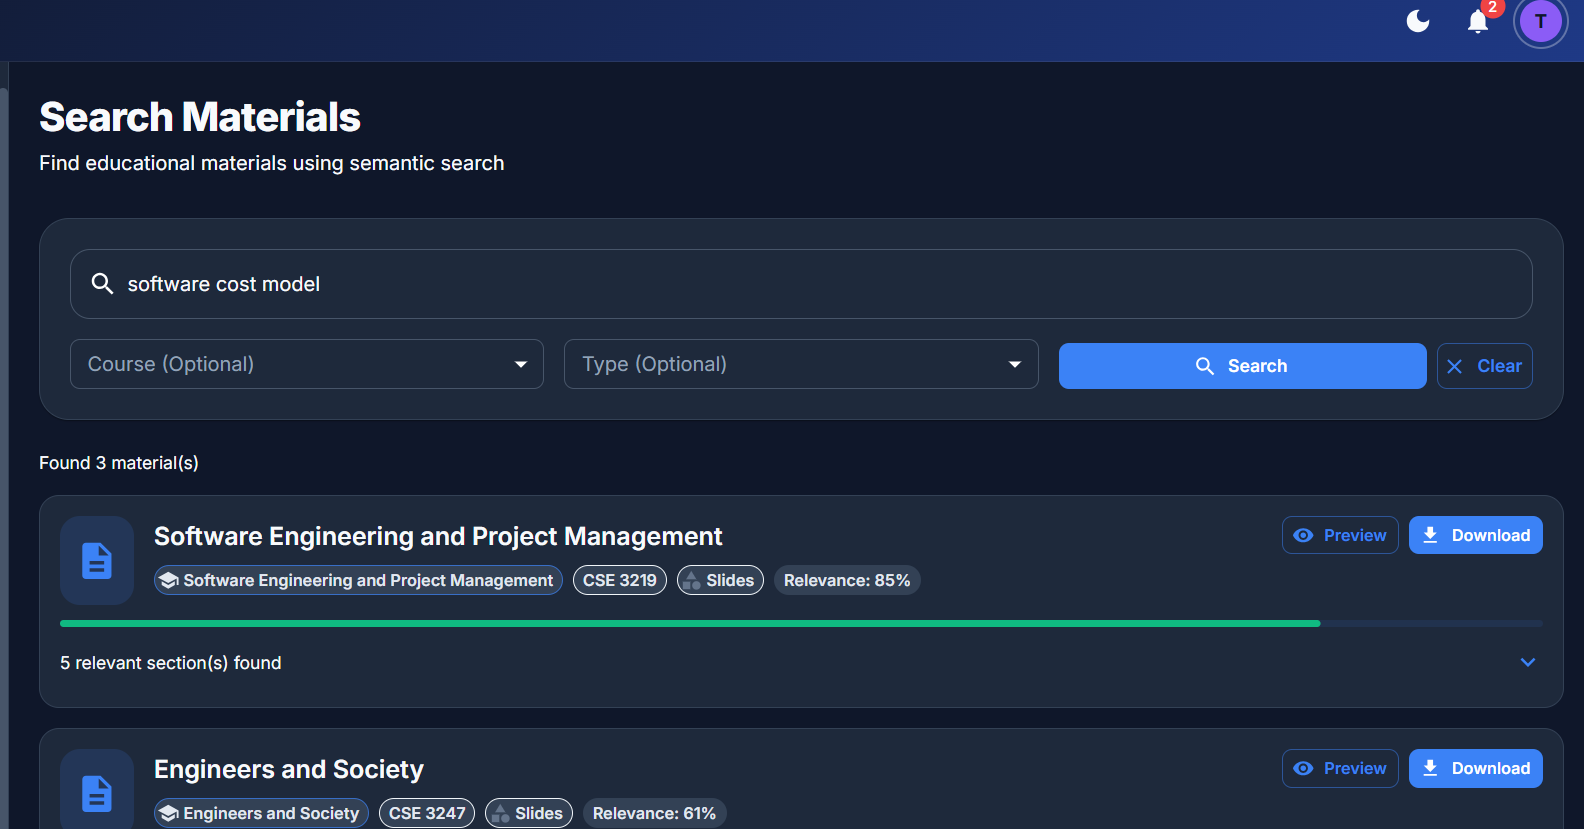
\includegraphics[width=\textwidth,height=0.31\textheight,keepaspectratio]{system_ss/semantic.png}
  \captionof{figure}{Semantic Search Interface}
  \label{fig:ss_search}
\end{minipage}\hfill
\begin{minipage}[t]{0.48\textwidth}
  \centering
  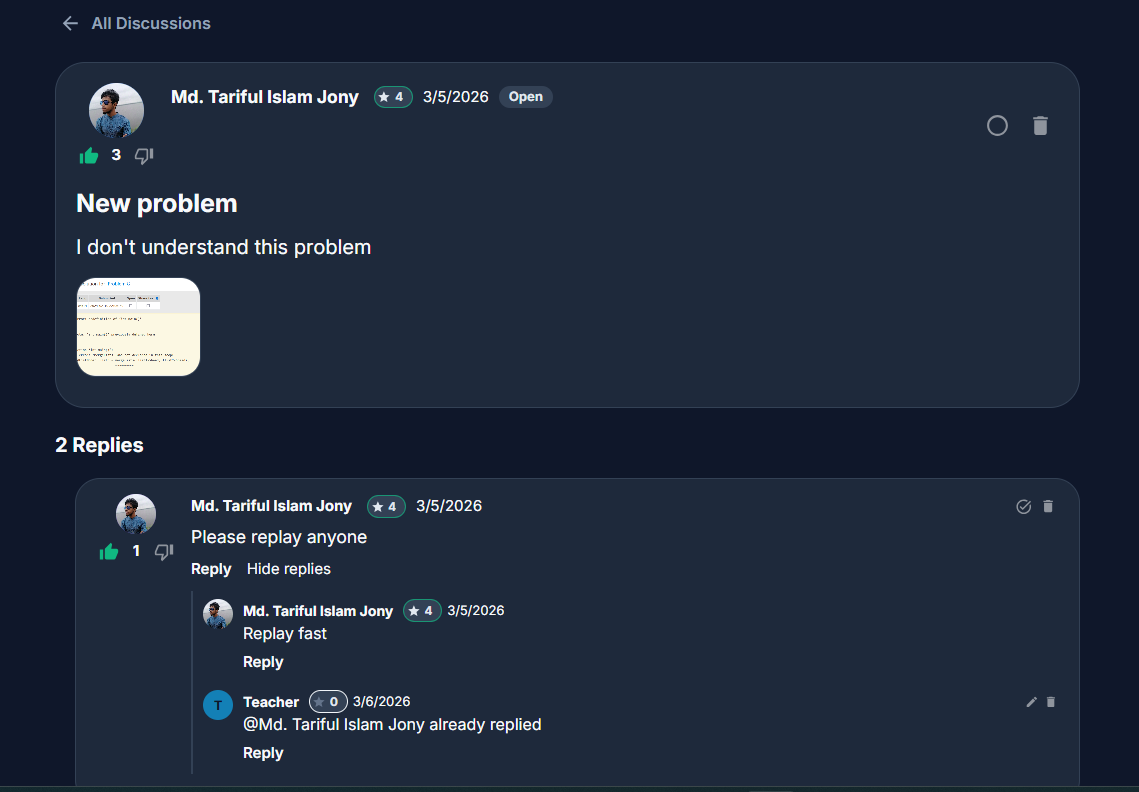
\includegraphics[width=\textwidth,height=0.31\textheight,keepaspectratio]{system_ss/discuss.png}
  \captionof{figure}{Discussion Forum Interface}
  \label{fig:ss_discussion}
\end{minipage}
\end{figure}
\clearpage

\begin{figure}[H]
\centering
\begin{minipage}[t]{0.48\textwidth}
  \centering
  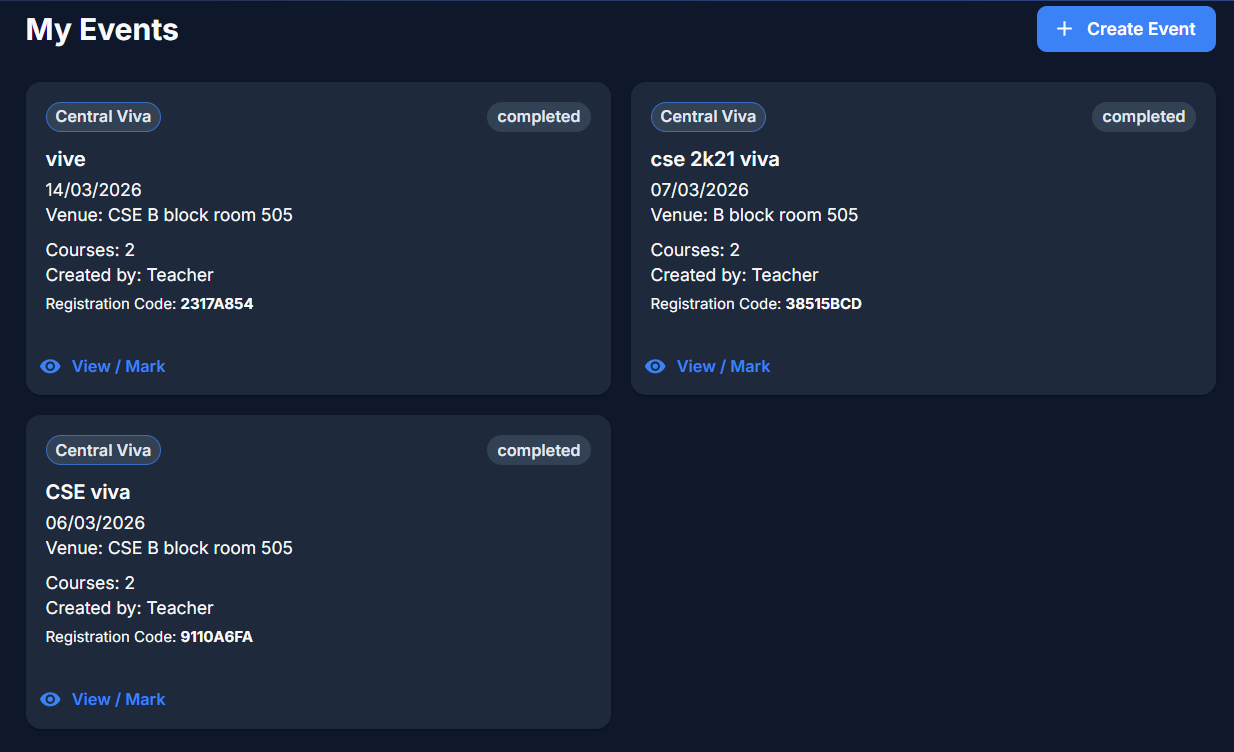
\includegraphics[width=\textwidth,height=0.31\textheight,keepaspectratio]{system_ss/event.png}
  \captionof{figure}{Academic Event Management Panel}
  \label{fig:ss_event}
\end{minipage}\hfill
\begin{minipage}[t]{0.48\textwidth}
  \centering
  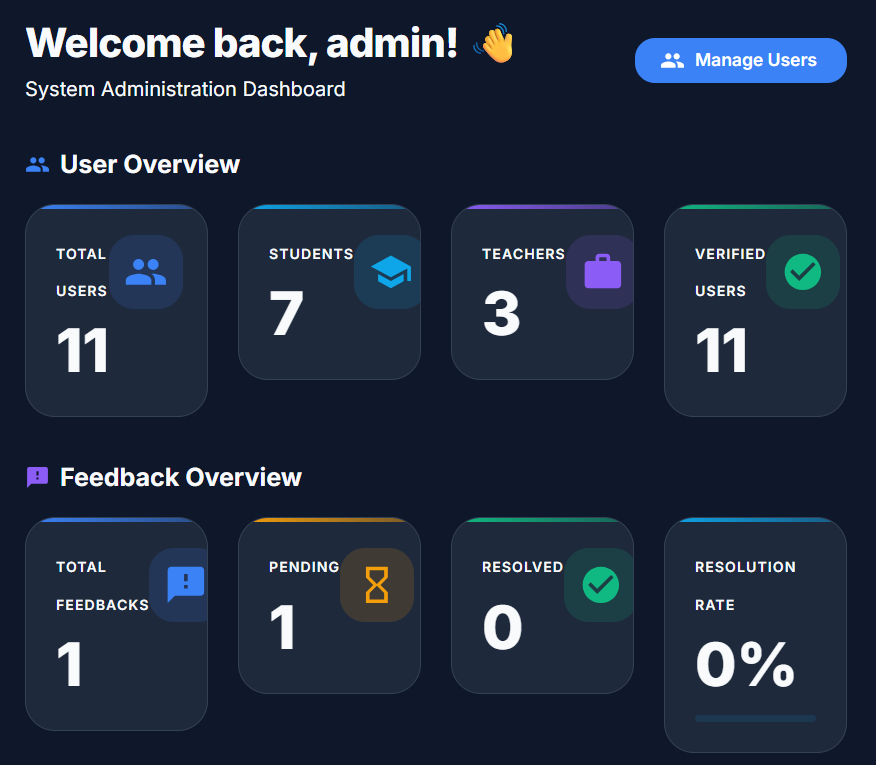
\includegraphics[width=\textwidth,height=0.31\textheight,keepaspectratio]{system_ss/admin_dash.png}
  \captionof{figure}{Admin Dashboard Overview}
  \label{fig:ss_admin_dash}
\end{minipage}
\end{figure}
\begin{figure}[H]
\centering
\begin{minipage}[t]{0.48\textwidth}
  \centering
  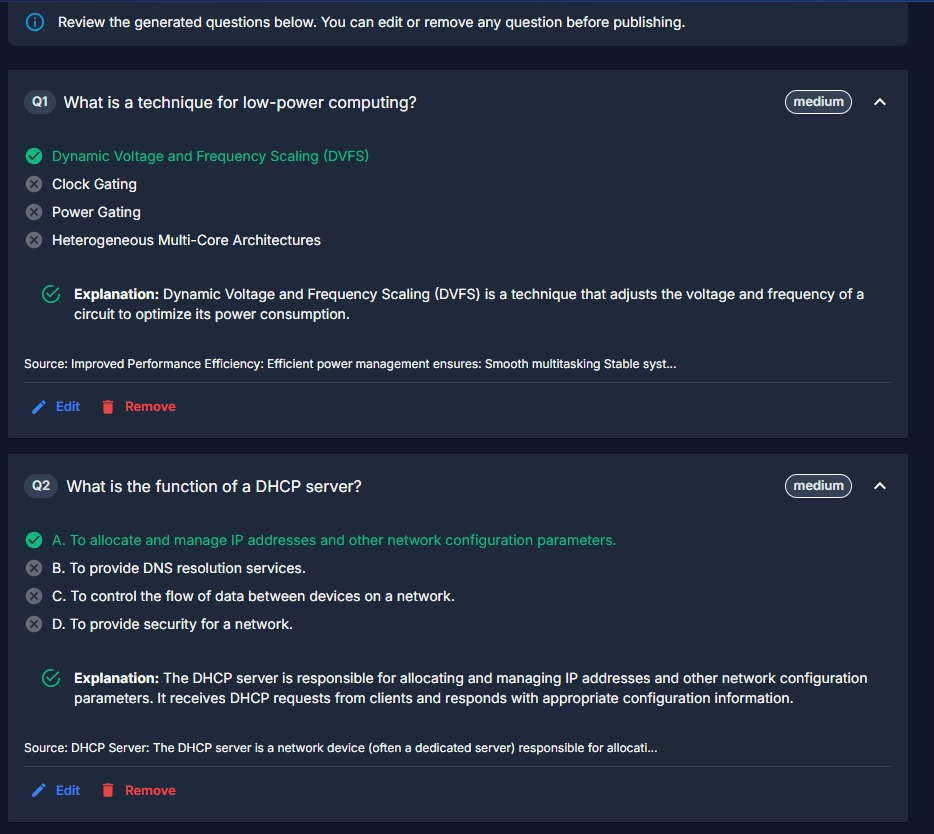
\includegraphics[width=\textwidth,height=0.31\textheight,keepaspectratio]{system_ss/ai_quiz.png}
  \captionof{figure}{AI Quiz Generation Interface}
  \label{fig:ss_ai_quiz}
\end{minipage}\hfill
\begin{minipage}[t]{0.48\textwidth}
  \centering
  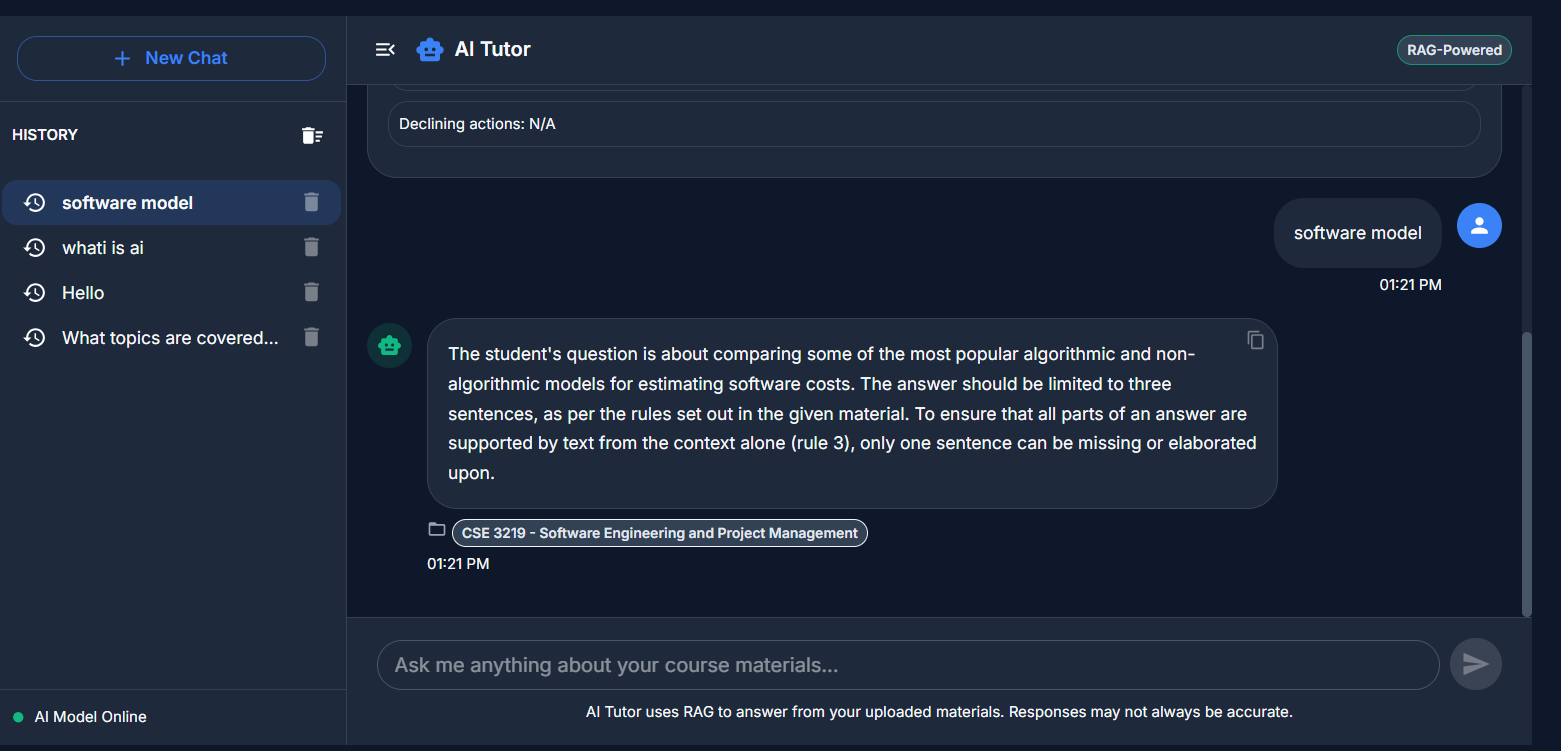
\includegraphics[width=\textwidth,height=0.31\textheight,keepaspectratio]{system_ss/ai_tutor.png}
  \captionof{figure}{AI Tutor Chat Interface}
  \label{fig:ss_ai_tutor}
\end{minipage}
\end{figure}

The student journey starts with institution-specific KUET email registration and OTP-based authentication. On successful login, the student is presented with a role-based dashboard highlighting enrolled courses, uncompleted assignments with due-date timers, and unread notifications. A student can enroll in a course by providing an eight-character course code as shared by the teacher. The student can view the course announcement stream with threaded comments, the list of assignments with indicators of per-submission status (Not Submitted / Submitted Late / Graded), the list of quizzes with the history and scores of attempts, the feed of materials limited to enrolled courses, and a discussion forum.

The semantic search interface presents a query bar at the top; results appear below as material cards with relevance score badges and expandable matching text excerpts. The student can also filter results by course. The RAG AI Tutor is accessible from a persistent tab; the chat session history is preserved in a collapsible sidebar. If the student asks a question that does not match a topic in the uploaded materials, the topic relevance gate returns the fallback phrase immediately, avoiding a confusing response from the LLM. The response UI includes citations to the source document, enabling the student to jump to the source material.

The Adaptive Recommendations page shows the student a ranked list of study materials alongside the per-topic performance scores that drove each recommendation. Each material card displays the topic tags it covers, a human-readable explanation (e.g., ``You scored 32\% on Memory Paging --- this material covers it in depth''), and a direct link to view or download the file.

The teacher user interface provides for material upload (automatic background text extraction, chunk embedding, and topic tag assignment), the AI quiz generator which creates draft MCQ questions from course slides in about 45 seconds per five questions, manual quiz creation (with questions and answer keys), assignment creation (with due dates and upload of result sheets), event creation (for vivas, presentations, with marks collected across courses), and teacher invitations to other teachers to access a course.

The administrator experience includes user and course management dashboards, feedback moderation queue with email notification sent to students, and the Synthetic Data Lab which populates namespaced test datasets (at user-specified scale: teachers, students, courses, materials, quizzes, and learning events in one go, with namespace-scoped cleanup).

\subsection{Quantitative Results}

\begin{table}[htbp]
\caption{Semantic Search Retrieval Evaluation Results (60-query manual test set)}
\label{tab:search_results}
\centering
\begin{tabular}{|l|c|c|}
\hline
\textbf{Retrieval Strategy} & \textbf{Precision@5} & \textbf{nDCG@10} \\
\hline
BM25 Keyword-Only (baseline) & 0.52 & 0.48 \\
Dense-Only (cosine similarity, no lexical gate) & 0.68 & 0.63 \\
Hybrid Dense+Lexical Gate (SyncAcademy) & \textbf{0.74} & \textbf{0.69} \\
\hline
\end{tabular}
\end{table}

\begin{table}[htbp]
\caption{RAG AI Tutor Evaluation Results (60-query manual test set)}
\label{tab:rag_results}
\centering
\begin{tabular}{|l|c|}
\hline
\textbf{Metric} & \textbf{Value} \\
\hline
Grounded answer rate (all sentences context-supported) & 0.87 \\
Partial out-of-context rate & 0.10 \\
Fallback trigger rate on explicitly off-topic queries & 0.93 \\
\hline
\end{tabular}
\end{table}

\begin{table}[htbp]
\caption{AI Quiz Generator Grounding Evaluation (200 generated questions across 5 courses)}
\label{tab:quiz_results}
\centering
\begin{tabular}{|l|c|}
\hline
\textbf{Metric} & \textbf{Value} \\
\hline
Questions passing grounding validation (key terms in source chunk) & 83\% \\
Questions discarded as ungrounded & 17\% \\
Average generation time (5 questions via \texttt{llama3.1}) & ${\sim}45$ seconds \\
\hline
\end{tabular}
\end{table}

\begin{table}[htbp]
\caption{Tag-Based Recommendation Evaluation (30 simulated student profiles, 5-topic course)}
\label{tab:rec_results}
\centering
\begin{tabular}{|l|c|c|}
\hline
\textbf{Condition} & \textbf{MRR} & \textbf{Precision@3} \\
\hline
Random baseline & 0.38 & 0.33 \\
Tag-only (no performance weighting) & 0.54 & 0.51 \\
Inverse-performance ranking (SyncAcademy) & \textbf{0.68} & \textbf{0.71} \\
\hline
\end{tabular}
\end{table}

\subsection{Analysis of Results}

The improvement achieved by hybrid retrieval over keyword-only is greatest when querying with vocabulary mismatch, for example, with the query ``how does TCP guarantee reliable delivery'' and the slide titled ``TCP acknowledgement and retransmission mechanism''. The lexical overlap gate lowers the false-positive rate from 21\% (cosine-only) to 10\% (manual evaluation), by gating out high-cosine-but-lexically-empty matches that resulted from proximity in embedding space in a general semantic sense but were not conceptually relevant.

For the RAG AI Tutor, the 10\% partial out-of-context error rate reflects the inherent difficulty of constraining a smaller open-source LLM. The 93\% fallback trigger rate on off-topic queries confirms that the topic relevance gate is the primary defence: the LLM is only invoked when the retrieved context genuinely contains the queried concept.

The 17\% discard rate of AI quiz questions reflects genuine LLM excursions beyond the source chunk. The $N+2$ chunk buffer per question generation ensures the desired number of questions is met, and the discard rate validates that the grounding check is functioning correctly and not simply rejecting well-formed questions.

For tag-based recommendations, the inverse-performance ranking outperforms both the random baseline and a pure tag-matching approach (which ignores performance history). The improvement is most pronounced for students with uneven topic profiles --- students who excel at some topics but have clear weaknesses in others benefit the most from performance-weighted ranking, whereas students with uniformly low or uniformly high performance see smaller gains.

\section{Objective Achieved}

The six objectives listed in Section~1.3 are all met. A full LMS with roles is running in production. The hybrid semantic search achieves a Precision@5 of 0.74, exceeding the target of 0.70. The RAG AI Tutor achieves an 87\% grounded answer rate, above the 0.85 target. The AI quiz generator reaches 83\% on the grounding pass rate, exceeding the 0.80 target. The tag-based recommendation system achieves an MRR of 0.68 and Precision@3 of 0.71, both above their targets. The system is deployed and publicly accessible online.

\section{Conclusion}

The implementation demonstrates the merit of hybrid semantic search over pure-lexical and pure-dense retrieval schemes, the effectiveness of the multi-stage context constraint in mitigating RAG hallucination for a smaller open-source LLM, the efficacy of the grounding validation in AI quiz generation, and the practical value of performance-weighted tag-based recommendation over unweighted content matching.

%============================================================
\chapter{Societal, Health, Environment, Safety, Ethical, Legal and Cultural Issues}
%============================================================

\section{Intellectual Property Considerations}

All materials uploaded for educational purposes remain the copyright of the teacher who uploaded them. SyncAcademy does not share materials outside of course members, and Cloudinary URLs are signed. The embedding process translates text into dense vectors which are stored internally; these vectors do not represent a reproduction of the original work, and are not exposed to users. The AI Tutor generates responses that include metadata from the source material, providing context and attributing authorship to the original source for the student.

The system is implemented using open-source code libraries, under the terms of their respective licences (MIT, Apache 2.0, BSD-3, BSD-2). It does not include proprietary data or models.

\section{Ethical Considerations}

The greatest ethical risk of an AI tutor is hallucination. SyncAcademy overcomes this with the multi-step RAG validation process: a topic filter gate keeps irrelevant questions from reaching the LLM; context-only prompting with a fallback phrase ensures no knowledge dumps; and a self-evaluation step can detect unfaithful answers. The system is deliberately designed not to guess.

A secondary ethical concern is the fairness of the recommendation system. Tag-based recommendations driven by quiz and assignment performance could disadvantage students who perform poorly on early assessments due to test anxiety or other transient factors, by persistently surfacing remedial material rather than advancing content. To mitigate this, the recency weighting in the performance score computation ensures that recent strong performance reduces the influence of earlier poor performance, and the teacher can override or adjust tag assignments on any material.

The Synthetic Data Lab has namespaced accounts, preventing synthetic users from contaminating institutional production data, and allows batch deletion, minimising test pollution risks.

\section{Safety Considerations}

Security constraints include: JWT token expiry for stateless session invalidation; bcrypt password hashing with cost factor 10; OTP-based email verification with KUET institutional addresses; role-based middleware guards on all protected API endpoints; Multer file type and size (50~MB) limits (PDF, DOCX, PPTX); signed Cloudinary URLs to restrict unauthorised access to files; and environment variable-only storage of all secrets with a \texttt{.env.example} template committed to the repository for onboarding purposes.

The Ollama LLM is a local process that is not publicly accessible. No student query text is sent to third parties locally. The only text data sent externally is chunk content and query text to the Hugging Face Inference API for embedding; system operators should review HuggingFace's data retention policy for compliance.

\section{Legal Considerations}

SyncAcademy retains KUET student email addresses, seven-digit student IDs, and student results (grades, marks, quiz scores). Data protection laws (e.g., national laws in Bangladesh) require the system be operated with a legal purpose for processing, retention schedules, and processes for data subject access and deletion. The current version of the system does not have an automated data deletion process; this is a requirement for use in a regulated environment.

Third-party providers (Cloudinary, Hugging Face, Render, MongoDB Atlas) have their own terms of service; SyncAcademy operators must abide by these when using these services for storing student data.

\section{Impact of the Project on Societal, Health, and Cultural Issues}

SyncAcademy lowers the cost of educational support by offering AI tutoring based on course-relevant materials to all students, regardless of ability to pay for private tutoring services. The AI Tutor's tight context constraint means that explanations are provided based on course content, ensuring that the tutoring matches the course instructor's judgement of what is important. The tag-based recommendation system encourages self-regulated learning strategies --- identifying weak topic areas and directing study time accordingly --- which have been shown to have long-term positive effects on academic performance.

There are no expected health effects. Potential second-order effects include the risk of screen fatigue due to prolonged use, and loss of problem-solving skills if students are over-reliant on the AI explanations. These concerns are addressed by the system's role as a supplement, the three-sentence limit of the AI Tutor's responses encouraging students to delve deeper, and the course context constraint, which limits students to only using the tutor within a specific course context.

\section{Impact of the Project on the Environment and Sustainability}

Local Ollama inference for LLM responding means no per-inference network round trips to remote AI services, greatly reducing the network and data-centre energy required for a large-scale deployment compared to cloud API inference. The system uses an energy-efficient sentence embedding model (\texttt{all-MiniLM-L6-v2}, 22 million parameters), one of the most efficient transformer-based embedding models, with many fewer floating-point operations than larger models. It runs on Render's shared runtime environment, which is more energy efficient due to data-centre economies of scale. No hardware is created for this project; the system uses existing cloud and developer hardware.

%============================================================
\chapter{Addressing Complex Engineering Problems and Activities}
%============================================================

\section{Complex Engineering Problems Associated with the Current Project}

\textbf{Suppression of hallucinations for a small open-source LLM.} Hallucination prevention is much more difficult for the \texttt{llama3.1} model running on Ollama than for large frontier models. In preliminary experiments the model routinely ignored simple context restrictions. To engineer an effective prompt, it was necessary to: explicitly identify and name every known loophole to the restriction in the system prompt; introduce a required fallback phrase to be used in the absence of sufficient context; impose a domain-specific topicality gate during the retrieval stage to avoid false-positive chunk sets; limit the answer to three sentences; and incorporate an optional LLM-as-a-judge self-check. Achieving the 87\% grounded answer rate required multiple rounds of qualitative analysis of prompt structure variants; this is a complex engineering problem because there is no analytic formula for the optimal prompt structure for a given model and task combination.

\textbf{Hybrid retrieval threshold tuning.} Setting the cosine similarity threshold $\tau_s$, token overlap ratio threshold $\tau_o$, and short-query variant $\tau_{o,\text{short}}$ requires a multi-dimensional optimisation of precision (to avoid false positives on off-topic queries) and recall (to avoid false negatives on relevant queries). Neither threshold is analytically derivable; values depend on the geometry of the embedding model, the vocabulary of the domain, and the length distribution of queries. The solution involved creating a manually labelled 60-query evaluation set with two annotators agreeing on relevance, a threshold sweep, and choosing values that optimise the harmonic mean of Precision@5 and recall@10 on a held-out set, while ensuring tolerable false positive rates on off-topic queries.

\textbf{Auto-tagging with sparse course taxonomies.} The material auto-tagging pipeline must assign meaningful topic tags to uploaded files even when the course TopicTaxonomy is sparse (few aliases defined) or when a material covers content adjacent to but not explicitly named in the taxonomy. Achieving reliable tagging in these conditions required the hybrid confidence scoring approach (combining alias overlap with semantic embedding similarity) and the conservative confidence threshold of 0.35, below which tags are withheld rather than forcing a possibly wrong label. The threshold was calibrated on a manually tagged set of 80 material chunks across four courses.

\textbf{Scalable per-chunk vector search in MongoDB.} Cosine similarity search in the application layer is $O(|\textit{MaterialChunk}|)$ in the number of documents. Several design iterations were required to produce a correct and workable implementation: pre-filtering to only the courses the user is enrolled in, reducing the candidate field substantially; projection queries (only the \texttt{chunkText} and \texttt{embedding} fields) to minimise payload size; a top-N limit (50 chunks) before grouping; and explicit query limits to restrict the size of the aggregation. This is a complex engineering exercise because the solution lies at the crossroads of database query optimisation, application caching strategy, and embedding design choices.

\section{Complex Engineering Activities Associated with the Current Project}

\textbf{Full-stack AI pipeline integration.} The integration of nine different AI-related components (Multer upload, Cloudinary storage, three-format text extraction --- pdf-parse, mammoth, officeparser --- text chunking, HuggingFace embedding API, MongoDB chunk persistence, cosine-similarity retrieval, auto-tagging, and Ollama text generation) into a single request-response pipeline, with progressive degradation for each component's error case (API rate limit, Ollama timeout, extraction failure, zero-retrieval result), demanded careful attention to error boundaries and fallbacks. This is a multi-system integration task which goes beyond merely implementing each component in isolation.

\textbf{Tag-based recommendation pipeline design.} The recommendation pipeline is a multi-stage ETL-style process: quiz and assignment events are mapped through topic tags to per-topic performance scores, which are then used to rank materials by inverse score. Ensuring that this pipeline remains correct across all edge cases --- students with no quiz history, materials with no tags, courses with no taxonomy defined, and the neutral prior fallback --- required careful defensive coding and integration testing across many simulated user profiles. The pipeline is also recency-sensitive: the exponential decay weighting ensures that the most recent interactions dominate, which requires consistent timestamp handling across quiz attempts, assignment submissions, and material interaction events.

\textbf{Role-based permission enforcement across a 25-route API.} Consistent role-based access control across all route modules (including asymmetric cases such as mark entry for a given event course by the assigned teacher only, co-teacher versus primary teacher, student-controlled reveal of an evaluated script) entailed careful middleware composition, review of the per-route permission matrix, and integration testing for corner cases. The academic event system's composite permission model (event author, course-assigned teacher, student, admin) provided the most intricate privilege intersection in the system.

%============================================================
\chapter{Conclusions}
%============================================================

\section{Summary}

SyncAcademy is a full-stack, AI-powered smart classroom management system that augments the traditional LMS framework by integrating semantic search, context-constrained RAG tutoring, AI quiz generation, and a tag-based adaptive recommendation system into academic processes. Powered by Node.js 18, React 18, MongoDB Atlas, Ollama, and the HuggingFace embedding API, the system offers student, teacher, and admin interfaces automatically authenticated from KUET domain emails. It replicates and extends the core Google Classroom feature set by providing course enrollment with automatically generated course codes, a rich stream of announcements with nested comment threads, assignment management with late work detection and result sheet export, a discussion forum with answer voting, an academic event management module for vivas and thesis defences, and an in-app notification system for 14 event types.

The three AI components deliver a hybrid search Precision@5 of 0.74, an RAG grounded answer rate of 87\%, an AI quiz grounding pass rate of 83\%, and a tag-based recommendation MRR of 0.68 --- all surpassing their respective target levels. The material auto-tagging pipeline produces topic tag assignments with a hybrid alias-overlap and embedding-similarity confidence score, enabling the recommendation engine to surface study materials targeting each student's weakest topic areas with full per-material explainability.

\section{Limitations}

The following limitations are acknowledged. First, vector search is conducted in application code without approximate nearest-neighbour indexing, and the material database is not large; performance may degrade as the corpus grows. Second, the 10\% partial out-of-context error rate in RAG responses suggests that the smaller \texttt{llama3.1} model occasionally goes out of context; prompt engineering for smaller models is less predictable than for frontier models. Third, the auto-tagging pipeline depends on the quality and completeness of the teacher-defined TopicTaxonomy; courses with sparse or missing taxonomies produce fewer and less accurate tag assignments. Fourth, tag-based recommendation was evaluated on simulated student profiles rather than real longitudinal student interaction data from KUET, which may not represent real-world performance distributions. Fifth, a data retention and deletion pipeline is not in place, and formal adherence to personal data laws is limited. Sixth, the system has not been load-tested for multiple concurrent user sessions, and it is unclear how it will perform during an academic peak period.

\section{Recommendations and Future Works}

Future work will focus on the following areas. Chunk-level vector storage can be moved into a dedicated vector database (e.g., Qdrant or Weaviate) to allow approximate nearest-neighbour search with millisecond response time on large document sets. Deploying the system for real KUET students would yield realistic quiz and assignment performance data for calibrating the recommendation engine on genuine learning outcomes and validating the tag confidence thresholds on real course taxonomies. A teacher-facing analytics dashboard showing per-topic class-level performance distributions, derived from the tag-based performance scores, would boost the educational value of the recommendation data for course planning. A data retention and deletion policy would enable full regulatory compliance. A Progressive Web App wrapper would allow mobile device access for students. Trialling task-specific fine-tuning of a smaller LLM using LoRA adapters on corpora related to the course would enhance RAG grounded answer rates without additional cost. Lastly, integration of AI-suggested related resources to the discussion forum when a question is posted would complete the loop from the forum to the semantic search and recommendation modules.

%============================================================
%  APPENDICES
%============================================================
\appendix

\chapter{REST API Endpoint Summary}

\begin{table}[htbp]
\caption{Key REST API Endpoints Implemented in SyncAcademy}
\label{tab:api}
\centering
\small
\begin{tabularx}{\textwidth}{|l|l|l|X|}
\hline
\textbf{Method} & \textbf{Endpoint} & \textbf{Auth / Role} & \textbf{Description} \\
\hline
POST & /api/auth/register & None & Register; role auto-detected from KUET email domain \\
POST & /api/auth/login & None & Login; returns signed JWT \\
POST & /api/auth/verify-otp & None & Verify OTP sent to institutional email \\
GET  & /api/courses & JWT & List courses (enrolled scope for students) \\
POST & /api/courses & Teacher & Create course; generates unique courseCode \\
POST & /api/enrollments/enroll & Student & Enroll using courseCode \\
POST & /api/materials/upload & Teacher & Upload file; triggers extraction, chunking, embedding, and auto-tagging \\
POST & /api/search & JWT & Hybrid semantic search over enrolled-course materials \\
POST & /api/chat & JWT & Send message to RAG AI Tutor \\
GET  & /api/chat/health & JWT & Check Ollama server availability \\
POST & /api/announcements & Teacher & Create announcement with attachments and links \\
POST & /api/assignments & Teacher & Create assignment with due date and attachments \\
POST & /api/assignments/:id/submit & Student & Submit file or text response \\
PUT  & /api/assignments/:id/submissions/:sid/grade & Teacher & Assign grade and feedback \\
POST & /api/quizzes/generate & Teacher & AI quiz generation from course material chunks \\



\hline
\end{tabularx}
\end{table}

\chapter{Environment Configuration Variables}

The backend requires the following environment variables in \texttt{backend/.env}:

\begin{itemize}[leftmargin=0.5in]
  \item \texttt{MONGODB\_URI} --- MongoDB Atlas connection string
  \item \texttt{JWT\_SECRET} --- Signing secret for JSON Web Tokens
  \item \texttt{CLOUDINARY\_CLOUD\_NAME}, \texttt{CLOUDINARY\_API\_KEY}, \texttt{CLOUDINARY\_API\_SECRET} --- Cloudinary credentials
  \item \texttt{HUGGINGFACE\_API\_KEY} --- HuggingFace Inference API key for sentence embeddings
  \item \texttt{OPENAI\_API\_KEY} --- Optional OpenAI embedding fallback
  \item \texttt{OLLAMA\_BASE\_URL} --- Ollama server URL (default: \texttt{http://localhost:11434})
  \item \texttt{EMAIL\_USER}, \texttt{EMAIL\_PASS} --- SMTP credentials for OTP email dispatch
  \item \texttt{RAG\_ENABLE\_SELF\_EVAL} --- \texttt{true}/\texttt{false} (default: \texttt{false})
  \item \texttt{RAG\_SELF\_EVAL\_THRESHOLD} --- Float 0--1 for self-evaluation pass threshold (default: 0.5)
  \item \texttt{RAG\_MAX\_RETRIES} --- Maximum generation retries after self-evaluation failure (default: 1)
  \item \texttt{SEARCH\_MIN\_SIMILARITY\_THRESHOLD} --- Minimum cosine similarity for search (default: 0.40)
  \item \texttt{SEARCH\_MIN\_HYBRID\_THRESHOLD} --- Minimum hybrid score (default: 0.42)
  \item \texttt{TAGGING\_CONFIDENCE\_THRESHOLD} --- Minimum confidence for auto-assigned topic tags (default: 0.35)
  \item \texttt{TAGGING\_ALIAS\_WEIGHT} --- Weight $\beta$ for alias overlap in tag confidence score (default: 0.6)
\end{itemize}

%============================================================
%  REFERENCES
%============================================================
\newpage


\renewcommand{\refname}{References}  % For article/report class
% OR
\renewcommand{\bibname}{References}  % For book/thesis class

\begin{thebibliography}{99}
\bibitem{moodle} M. Dougiamas and P. C. Taylor, ``Moodle: Using Learning Communities to Create an Open Source Course Management System,'' in \textit{Proc. World Conf. Educational Multimedia, Hypermedia and Telecommunications (ED-MEDIA)}, 2003, pp. 171--178.

\bibitem{siemens} G. Siemens and P. Long, ``Penetrating the Fog: Analytics in Learning and Education,'' \textit{EDUCAUSE Review}, vol. 46, no. 5, pp. 30--32, Sep./Oct. 2011.

\bibitem{bert} J. Devlin, M.-W. Chang, K. Lee, and K. Toutanova, ``BERT: Pre-training of Deep Bidirectional Transformers for Language Understanding,'' in \textit{Proc. Conf. North American Chapter of the ACL: Human Language Technologies (NAACL-HLT)}, 2019, pp. 4171--4186.

\bibitem{dpr} V. Karpukhin, B. Oguz, S. Min, P. Lewis, L. Wu, S. Edunov, D. Chen, and W. Yih, ``Dense Passage Retrieval for Open-Domain Question Answering,'' in \textit{Proc. Conf. Empirical Methods in Natural Language Processing (EMNLP)}, 2020, pp. 6769--6781.

\bibitem{sbert} N. Reimers and I. Gurevych, ``Sentence-BERT: Sentence Embeddings Using Siamese BERT-Networks,'' in \textit{Proc. Conf. Empirical Methods in Natural Language Processing (EMNLP-IJCNLP)}, 2019, pp. 3982--3992.

\bibitem{sparse_dense} Y. Luan, J. Eisenstein, K. Toutanova, and M. Collins, ``Sparse, Dense, and Attentional Representations for Text Retrieval,'' \textit{Trans. Assoc. Comput. Linguistics}, vol. 9, pp. 329--345, 2021.

\bibitem{rag} P. Lewis, E. Perez, A. Piktus, F. Petroni, V. Karpukhin, N. Goyal, H. K{\"u}ttler, M. Lewis, W. Yih, T. Rockt{\"a}schel, S. Riedel, and D. Kiela, ``Retrieval-Augmented Generation for Knowledge-Intensive NLP Tasks,'' in \textit{Advances in Neural Information Processing Systems (NeurIPS)}, vol. 33, 2020, pp. 9459--9474.

\bibitem{replug} W. Shi, S. Min, M. Yasunaga, M. Seo, R. James, M. Lewis, L. Zettlemoyer, and W. Yih, ``REPLUG: Retrieval-Augmented Language Model Pre-Training,'' \textit{arXiv preprint arXiv:2301.12652}, 2023.

\bibitem{tagging} L. B. Marinho, A. Nanopoulos, L. Schmidt-Thieme, R. J{\"a}schke, A. Hotho, G. Stumme, and P. Symeonidis, ``Social Tagging Recommender Systems,'' in \textit{Recommender Systems Handbook}, F. Ricci, L. Rokach, B. Shapira, and P. B. Kantor, Eds. Boston, MA: Springer, 2011, pp. 615--644.

\bibitem{collab} J. S. Breese, D. Heckerman, and C. Kadie, ``Empirical Analysis of Predictive Algorithms for Collaborative Filtering,'' in \textit{Proc. 14th Conf. Uncertainty in Artificial Intelligence (UAI)}, 1998, pp. 43--52.

\bibitem{hybrid} R. Burke, ``Hybrid Recommender Systems: Survey and Experiments,'' \textit{User Modeling and User-Adapted Interaction}, vol. 12, no. 4, pp. 331--370, 2002.

\bibitem{bm25} S. Robertson and H. Zaragoza, ``The Probabilistic Relevance Framework: BM25 and Beyond,'' \textit{Foundations and Trends in Information Retrieval}, vol. 3, no. 4, pp. 333--389, 2009.
\end{thebibliography}

\end{document}
